\documentclass[10pt,twocolumn]{article}

\usepackage[a4paper,margin=0.70in]{geometry}
\usepackage{parskip}
\usepackage{amsmath}
\usepackage{amssymb}
\usepackage{graphicx}
\usepackage{booktabs}
\usepackage{caption}
\usepackage{float}
\usepackage[backend=bibtex,style=authoryear,maxbibnames=99]{biblatex}
\addbibresource{references.bib}

\setlength{\columnsep}{0.22in}
\setlength{\parskip}{2pt}
\setlength{\parindent}{0pt}
\sloppy

\graphicspath{
  {/Users/marcotiongson/Documents/fuel-abemis/Mini-Project/Agricultural Machinery Inventory from ABEMIS/Regression Parameters Output V3/}
  {/Users/marcotiongson/Documents/fuel-abemis/Mini-Project/Agricultural Machinery Inventory from ABEMIS/Analytics Output V2/}
}

\begin{document}

\twocolumn[
\begin{center}
{\large \textbf{Pilot Machine Learning Model for Fuel Requirement Estimation in Agricultural Mechanization}}\par
\vspace{4pt}
Ronald Melvin R. Rosas and Marcus Rafael Tiongson\par
\vspace{2pt}
{\small University of the Philippines, Diliman\par
\vspace{2pt}
May 2026\par}
\end{center}
\vspace{10pt}
]

%% ─────────────────────────────────────────────────────────────────────────────
\section*{Abstract}
%% ─────────────────────────────────────────────────────────────────────────────

This study develops a pilot machine learning model for estimating fuel requirements of agricultural machinery in the Philippines. A corpus of 378 cleaned training records was assembled from Agricultural Machinery Testing and Evaluation Center (AMTEC) PDF test reports and used to train two models: a Multiple Linear Regression (OLS) baseline and a Random Forest (RF) Regressor. Eight features were used for the RF model---five numeric and three categorical-encoded. On a held-out test set of 76 records, the RF achieves R\textsuperscript{2}\,=\,0.911, MAE\,=\,1.09\,L/h, and RMSE\,=\,1.61\,L/h, substantially outperforming the OLS baseline. SHAP feature-importance analysis reveals that rated engine power (\texttt{power\_kw}) dominates at approximately 76\% of total importance, consistent with the fuel--power proportionality established in the literature. The trained model was applied to score the Agricultural and Biosystems Engineering Management Information System (ABEMIS) national inventory, successfully predicting fuel requirements for 172,265 of 246,741 fuel-relevant records (70\%) across all 17 Philippine regions, enabling data-driven national mechanization planning.

%% ─────────────────────────────────────────────────────────────────────────────
\section*{I. Introduction}
%% ─────────────────────────────────────────────────────────────────────────────

Fuel consumption is a critical cost driver in agricultural mechanization and directly affects operational efficiency and sustainability. In the Philippines, fuel requirement estimation is typically based on generalized coefficients or static assumptions that do not account for variability in machine characteristics, field conditions, and operational practices \parencite{domsch1999fuel}.

Traditional engineering-based models provide approximate estimates but are limited in capturing nonlinear relationships among variables such as engine power, implement load, operation type, and field conditions. These models assume deterministic relationships that hold under standardized controlled test conditions; however, actual deployment across the diverse agro-ecological zones of the Philippines introduces variability that fixed coefficients cannot represent \parencite{briones2021philippine}.

The Agricultural Machinery Testing and Evaluation Center (AMTEC) has accumulated decades of standardized test reports covering a range of machinery types, engine capacities, and operational configurations. Simultaneously, the Bureau of Agricultural and Fisheries Engineering (BAFE) maintains the Agricultural and Biosystems Engineering Management Information System (ABEMIS), a national registry of distributed agricultural machinery. Despite the availability of these datasets, no systematic data-driven fuel estimation framework has been applied to link AMTEC performance data with ABEMIS inventory records.

With the increasing availability of agricultural datasets and the maturation of machine learning tools, it is now feasible to develop predictive models that improve estimation accuracy and support data-driven mechanization planning. This study proposes and evaluates a pilot machine learning model for estimating fuel requirements of selected agricultural machinery operations using structured operational data from AMTEC, enriched with deployment context from ABEMIS.

%% ─────────────────────────────────────────────────────────────────────────────
\section*{II. Problem Statement}
%% ─────────────────────────────────────────────────────────────────────────────

Current approaches to estimating fuel consumption in agricultural machinery are:
\begin{itemize}
  \item \textbf{Based on static or generalized coefficients} --- fuel requirement tables and engineering formulas apply global constants that are not derived from or validated against local Philippine field conditions.
  \item \textbf{Not localized to actual conditions} --- existing estimates ignore regional variability, machinery age, deployment scale, and crop-stage timing, all of which affect actual fuel demand in practice.
  \item \textbf{Unable to capture nonlinear interactions} --- deterministic formulas treat fuel consumption as a linear function of one or two inputs (typically engine power and area), missing the complex interactions among power, machinery type, operational mode, and deployment context.
\end{itemize}

As a result, there is a need for a data-driven model that can predict fuel consumption more accurately, adapt to different machine types and operations, and support improved decision-making in mechanized Philippine agriculture.

%% ─────────────────────────────────────────────────────────────────────────────
\section*{III. Objectives}
%% ─────────────────────────────────────────────────────────────────────────────

\textbf{General Objective:} To develop and evaluate a machine learning model for estimating fuel requirements of selected agricultural machinery operations using AMTEC test data and ABEMIS inventory context.

\textbf{Specific Objectives:}
\begin{itemize}
  \item Identify key variables affecting fuel consumption in Philippine agricultural machinery;
  \item Develop a baseline OLS regression model with group-level fallback hierarchy;
  \item Implement a Random Forest Regressor trained on the same feature set;
  \item Compare the two models using R\textsuperscript{2}, MAE, and RMSE on a held-out test set; and
  \item Perform feature-importance analysis using SHAP (global) and LIME (local) interpretability methods.
\end{itemize}

%% ─────────────────────────────────────────────────────────────────────────────
\section*{IV. Scope and Delimitation}
%% ─────────────────────────────────────────────────────────────────────────────

The study is limited to fuel consumption data extracted from AMTEC PDF test reports and machinery deployment records from ABEMIS. The target variable is fuel consumption in liters per hour (L/h) as reported in standardized AMTEC test conditions. The ABEMIS scoring pipeline applies the trained model to national inventory records to produce region-level fuel requirement estimates.

The cropping calendar from the Regional Agricultural Engineering Division (RAED) was identified as a planned time-dimension predictor representing crop stage and seasonal context. However, the RAED cropping calendar dataset was not yet acquired during the study period and its integration is deferred to future work.

The study excludes real-time sensor acquisition, GPS-based field tracking, full mechanization system simulation, and production-system deployment. The 247 AMTEC test reports that exist as scanned image PDFs (non-searchable) were not extractable with the current PyMuPDF text-extraction pipeline; OCR-based ingestion of these reports is deferred pending a Tesseract installation on the processing environment.

%% ─────────────────────────────────────────────────────────────────────────────
\section*{V. Review of Related Literature}
%% ─────────────────────────────────────────────────────────────────────────────

\subsection*{A. Fuel Consumption Theory}

Fuel requirement estimation in agricultural mechanization is based on the relationship between engine power, implement load, and operational efficiency. Fuel consumption is generally proportional to the power requirement of the machine during operation, making it a practical indicator of energy demand \parencite{domsch1999fuel}. Standardized measurement procedures have been developed to characterize this relationship under controlled test conditions, enabling comparison across machine types and power classes.

However, fuel consumption is not determined solely by engine characteristics. It is influenced by implement type, soil conditions, machine configuration, and operational mode. These relationships indicate that fuel estimation is a multivariate problem, and that single-variable engineering formulas can systematically underperform when applied outside their calibration conditions.

\subsection*{B. Empirical Modeling}

Empirical studies show that fuel consumption varies significantly under actual operating conditions. Analysis by \textcite{philmech_harvesters} of commercially available rice combine harvesters demonstrates that fuel consumption is closely related to engine power, field efficiency, and operational parameters including crop variety and moisture content. The Philippine Agricultural Engineering Standard \parencite{pnspaes148} establishes the tractor test procedure that underlies AMTEC reporting, linking rated power and field performance to standardized fuel measurements.

These empirical baselines confirm that while power is the primary determinant, secondary factors modulate actual consumption in ways that motivate a multivariate modeling approach.

\subsection*{C. Real-World Variability}

Real-world studies further emphasize that fuel consumption varies across agricultural systems and operating environments. \textcite{agaton2024solar} report, in the context of irrigation systems, that diesel fuel use is affected by soil type, environmental conditions, crop water requirements, distance to water source, and system efficiency. Although focused on irrigation rather than field machinery, this finding supports the argument that fuel use is context-dependent and that static coefficients cannot generalize across the heterogeneous conditions of Philippine agriculture.

\subsection*{D. Mechanization and Structural Context}

Agricultural mechanization increases productivity but also raises energy demand. Mechanization level, often measured in horsepower per hectare, reflects the degree of energy input in agricultural production \parencite{bautista2024enhancing}. Fuel and maintenance costs are major operational barriers faced by farmers, affecting sustainability and mechanization adoption rates \parencite{espino2024mechanization}.

Broader structural constraints---including policy fragmentation, limited financing, and post-harvest infrastructure gaps---also affect resource use and operational efficiency \parencite{ichwandiani2025industry, briones2021philippine}. Historical assessments of the Philippine agricultural machinery industry \parencite{itc2010machinery, jica1986philippines} document the evolution of mechanization from externally funded programs toward domestically driven adoption, setting the institutional context within which AMTEC and BAFE data originate.

\subsection*{E. Research Gap}

Existing approaches to fuel estimation rely largely on deterministic formulas, fixed coefficients, and controlled assumptions. These approaches have limited adaptability across varying field conditions and do not capture interactions among machine, operation, field, and effort-related variables. No prior study has applied machine learning to link AMTEC standardized test data with ABEMIS national inventory records to produce region-level fuel requirement estimates. The present study addresses this gap through a comparative OLS and Random Forest modeling approach with SHAP and LIME interpretability analysis.

%% ─────────────────────────────────────────────────────────────────────────────
\section*{VI. Conceptual Framework}
%% ─────────────────────────────────────────────────────────────────────────────

Fuel consumption is modeled as a function of four categories of variables:

\[
FC = f\!\left(
\begin{array}{l}
\text{Machine Characteristics,}\\
\text{Operation Characteristics,}\\
\text{Field/Location Conditions,}\\
\text{Operational Effort}
\end{array}
\right)
\]

The target variable is fuel consumption in L/h as recorded in AMTEC test conditions. The predictor variables in the implemented model are:

\begin{itemize}
  \item \textbf{Machine:} \texttt{power\_kw} (rated engine power in kW), \texttt{machinery\_type} (categorical), \texttt{machinery\_family} (categorical), \texttt{fuel\_type} (categorical)
  \item \textbf{Operation/Effort:} operating characteristics derived from AMTEC test analytics (encoded as numeric features)
  \item \textbf{Field/Context:} \texttt{abemis\_total\_count} (total national inventory count for the machinery type), \texttt{abemis\_region\_breadth} (number of regions where the type is deployed), \texttt{abemis\_dominant\_region\_share} (share held by the top deployment region)
  \item \textbf{Time (deferred):} crop stage and seasonal indicators from the RAED cropping calendar --- not yet integrated; reserved for future work
\end{itemize}

This framework captures machine-level physical determinants as primary predictors, with ABEMIS deployment-context features providing secondary structural information about the national inventory landscape.

%% ─────────────────────────────────────────────────────────────────────────────
\section*{VII. Dataset Description}
%% ─────────────────────────────────────────────────────────────────────────────

\subsection*{A. AMTEC Test Reports}

AMTEC machinery test reports (available at \texttt{https://bit.ly/AMTECTestReports2026}) provide the primary source of fuel consumption measurements. Reports cover field machinery, harvesters, dryers, and other mechanization equipment tested under standardized protocols \parencite{pnspaes148}. Text-searchable PDFs were processed using PyMuPDF to extract fuel consumption (L/h), rated engine power (kW), machinery type, fuel type, field efficiency, operating area, and operating time. After extraction, unit standardization, and outlier filtering, 378 clean records were retained as the training and test corpus.

\subsection*{B. ABEMIS Inventory}

The Agricultural and Biosystems Engineering Management Information System (ABEMIS), accessible at \texttt{https://abemis.bafe.gov.ph/user/login}, is maintained by BAFE and records the national distribution of agricultural machinery by region, municipality, barangay, and recipient type. After filtering for fuel-relevant records (machinery types that consume liquid fuel during operation), 246,741 records were identified across all 17 Philippine regions. Three ABEMIS-derived context features were engineered per machinery type: total inventory count, regional breadth, and dominant-region share.

\subsection*{C. RAED Cropping Calendar (Deferred)}

The Regional Agricultural Engineering Division cropping calendar was identified as the source of time-dimension predictors (crop stage, planting/harvesting window) that would link fuel demand to the agricultural season. The RAED dataset was not acquired during the study period. The data gathering instrument (\emph{Data Gathering Form for Cropping Calendar, AO 07-22-2022}) is on file but the dataset itself is pending. Integration is deferred to future work.

\subsection*{D. Feature Summary}

The Random Forest model uses 8 features:
\begin{itemize}
  \item \textbf{Numeric (5):} \texttt{power\_kw}, \texttt{abemis\_total\_count}, \texttt{abemis\_region\_breadth}, \texttt{abemis\_dominant\_region\_share}, and one additional operating characteristic derived from AMTEC test analytics
  \item \textbf{Categorical-encoded (3):} \texttt{machinery\_type}, \texttt{machinery\_family}, \texttt{fuel\_type}
  \item \textbf{Target:} fuel consumption (L/h)
\end{itemize}

%% ─────────────────────────────────────────────────────────────────────────────
\section*{VIII. Methodology}
%% ─────────────────────────────────────────────────────────────────────────────

\subsection*{A. Pipeline Overview}

The modeling pipeline proceeds as follows:
\begin{enumerate}
  \item \textbf{PDF Extraction} --- PyMuPDF (\texttt{fitz}) is used to extract structured text from text-searchable AMTEC PDFs. Scanned image PDFs are flagged for deferred OCR processing.
  \item \textbf{Unit Standardization} --- Horsepower values are converted to kW; area units normalized to hectares; time to hours; fuel to liters.
  \item \textbf{Outlier Filtering} --- Records with implausible fuel consumption values (e.g., negative, zero, or extreme outliers by machinery type) are removed using interquartile-range-based filtering at the machinery-type level.
  \item \textbf{Feature Engineering} --- ABEMIS context features are joined to AMTEC records by \texttt{machinery\_type} key. Categorical variables are label-encoded for RF input.
  \item \textbf{Train/Test Split} --- An 80/20 stratified split (378 total records; 302 training, 76 test) is applied. Stratification is on \texttt{machinery\_family}.
  \item \textbf{Model Training} --- OLS baseline and RF Regressor are fitted on the training set.
  \item \textbf{Interpretability} --- SHAP and LIME analyses are performed on the RF model.
  \item \textbf{ABEMIS Scoring} --- The trained RF model scores all 246,741 ABEMIS fuel-relevant records to produce region-level fuel estimates.
\end{enumerate}

\subsection*{B. Baseline OLS Model}

A Multiple Linear Regression baseline is implemented with \texttt{power\_kw} as the primary predictor. Both linear and quadratic enrichments of \texttt{power\_kw} are evaluated. To handle machinery-type heterogeneity, a group-level fallback hierarchy is applied: the model first uses a \texttt{machinery\_type}-level fit; if insufficient data exist for a given type ($n < 5$), it falls back to the \texttt{machinery\_family}-level fit; and if that also fails, it falls back to the global (all-machinery) model. This hierarchy produces a set of scoped OLS models evaluated against the same holdout test set.

\subsection*{C. Random Forest Regressor}

A Random Forest Regressor is trained using scikit-learn defaults (100 estimators, no maximum depth constraint, minimum samples split of 2). All 8 features are used. Label encoders are fitted per categorical feature on the training set and applied to both test and ABEMIS scoring sets. The model is evaluated on the 76-record holdout set.

\subsection*{D. Interpretability}

SHAP TreeExplainer is applied to the trained RF model to compute global feature importance (mean absolute SHAP value per feature) and per-sample SHAP contributions. A beeswarm plot visualizes the distribution of SHAP values across all test samples. LIME tabular explainer generates local explanations for 10 selected example records, identifying which features most influenced each individual prediction. Results are exported to \texttt{SHAP\_Analysis.xlsx} and \texttt{LIME\_Explanations.xlsx}.

\subsection*{E. Evaluation Metrics}

Model performance is evaluated using:
\[
R^2 = 1 - \frac{\sum_i (y_i - \hat{y}_i)^2}{\sum_i (y_i - \bar{y})^2}
\]
\[
\mathrm{MAE} = \frac{1}{n}\sum_{i=1}^{n} |y_i - \hat{y}_i|
\]
\[
\mathrm{RMSE} = \sqrt{\frac{1}{n}\sum_{i=1}^{n}(y_i - \hat{y}_i)^2}
\]

where $y_i$ is the actual fuel consumption, $\hat{y}_i$ is the model prediction, $\bar{y}$ is the sample mean, and $n = 76$ for the holdout set.

%% ─────────────────────────────────────────────────────────────────────────────
\section*{IX. Results}
%% ─────────────────────────────────────────────────────────────────────────────

\subsection*{A. Model Comparison}

Table~1 presents the holdout evaluation metrics for the OLS and Random Forest models. The Random Forest substantially outperforms all OLS variants across all three metrics.

\begin{table}[H]
\centering
\captionsetup{font=small}
\caption{OLS vs.\ Random Forest holdout metrics ($n = 76$)}
\label{tab:metrics}
\small
\begin{tabular}{lccc}
\toprule
\textbf{Model} & \textbf{R\textsuperscript{2}} & \textbf{MAE (L/h)} & \textbf{RMSE (L/h)} \\
\midrule
OLS Global Linear         & 0.761 & 1.683 & 2.640 \\
OLS Hierarchical Fallback & 0.722 & 1.872 & 2.847 \\
\textbf{Random Forest}    & \textbf{0.911} & \textbf{1.090} & \textbf{1.611} \\
\bottomrule
\end{tabular}
\end{table}

\vspace{2pt}
{\footnotesize Note: Hierarchical OLS uses a per-machinery-type fallback chain (type $\to$ family $\to$ global). Random Forest 5-fold cross-validation mean: R\textsuperscript{2}\,=\,0.895, MAE\,=\,1.08, RMSE\,=\,1.77. Full results are in \texttt{OLS\_vs\_RF\_Comparison.xlsx}.}

\subsection*{B. SHAP Feature Importance}

SHAP analysis (Figures~1--2 in Appendix~A) reveals that \texttt{power\_kw} dominates feature importance at approximately 76\% of total mean absolute SHAP value. The three ABEMIS context features (\texttt{abemis\_total\_count}, \texttt{abemis\_region\_breadth}, \texttt{abemis\_dominant\_region\_share}) contribute approximately 3.5\% combined, consistently appearing in the lower half of the SHAP bar chart but with directionally coherent contributions visible in the beeswarm plot. Categorical features (\texttt{machinery\_type}, \texttt{machinery\_family}, \texttt{fuel\_type}) account for the remainder.

The dominance of \texttt{power\_kw} is consistent with the physical fuel--power proportionality established by \textcite{domsch1999fuel}: higher engine power ratings require more fuel to sustain operation regardless of machinery type.

\subsection*{C. LIME Local Explanations}

LIME tabular explainer was applied to 10 example records (Appendix~C). Across all 10 instances, \texttt{power\_kw} appeared as the top local contributor in 9 out of 10 cases. Machinery type and fuel type provided secondary adjustments, particularly for records involving dryers and non-diesel fuel types. The LIME results are consistent with the global SHAP picture, providing per-record interpretability for model validation.

\subsection*{D. ABEMIS National Scoring}

The trained RF model was applied to all 246,741 fuel-relevant ABEMIS records to produce regional fuel requirement estimates:
\begin{itemize}
  \item \textbf{Successfully scored:} 172,265 records (70\%) across all 17 Philippine regions
  \item \textbf{Excluded --- missing Rated Power:} 62,808 records (${\sim}25\%$) where the ABEMIS machinery entry did not carry a parseable rated power value
  \item \textbf{Excluded --- unmappable machinery type:} 11,668 records (${\sim}5\%$) where the ABEMIS machinery type could not be mapped to an AMTEC-covered type
\end{itemize}

Regional fuel estimates and dominant machinery families are reported in \texttt{ABEMIS\_Regional\_Fuel\_Estimates.xlsx}. Mobile field machinery (tractors, tillers) and harvest machinery (combine harvesters, reapers) account for the largest aggregate regional fuel estimates, consistent with their dominant share of the ABEMIS inventory.

%% ─────────────────────────────────────────────────────────────────────────────
\section*{X. Discussion}
%% ─────────────────────────────────────────────────────────────────────────────

\subsection*{A. Primacy of Engine Power}

The dominant contribution of \texttt{power\_kw} (${\sim}76\%$ SHAP importance) confirms the fundamental physical relationship between engine capacity and fuel demand \parencite{domsch1999fuel}. This result holds across all SHAP analysis levels (global bar chart, beeswarm distribution, and individual LIME explanations), providing high confidence in the model's physical coherence. The quadratic OLS enrichment of \texttt{power\_kw} also improved OLS performance over the linear baseline, further validating the nonlinear power--fuel relationship.

\subsection*{B. ABEMIS Context Features}

The three ABEMIS deployment-context features contribute a small but consistent 3.5\% of total SHAP importance. This suggests that knowledge of how widely and densely a machinery type is deployed across the country provides marginal but real predictive value, possibly capturing the fact that machinery types with higher national inventory counts tend to be better-maintained or operated at higher utilization rates. This contribution is not large enough to substitute for direct power measurement but adds value in scoring scenarios where power alone is insufficient.

\subsection*{C. Limitations}

Several limitations constrain the scope and generalizability of the current results:

\begin{itemize}
  \item \textbf{Scanned PDFs:} Approximately 247 AMTEC test report files exist as scanned image PDFs not extractable by PyMuPDF. Installation of Tesseract OCR is pending. Successful OCR of these reports is expected to increase the training corpus from 378 to approximately 500--550 records, potentially improving model stability for underrepresented machinery types.

  \item \textbf{RAED cropping calendar unavailable:} The time-dimension predictor (crop stage, planting/harvest window) could not be incorporated because the RAED dataset was not yet acquired. This limits the model's ability to account for seasonal load variations.

  \item \textbf{Missing Rated Power in ABEMIS:} Approximately 25\% of ABEMIS records (62,808 rows) carry no parseable Rated Power value, making them unscorable by the current model. Imputation or supplementary data linkage would be required to recover these rows.

  \item \textbf{Machinery-type mapping gaps:} Certain ABEMIS machinery types (e.g., corn mill) were approximated using the nearest AMTEC-tested proxy (e.g., rice mill). These proxy mappings introduce uncertainty and account for the 11,668 currently-unmapped records.
\end{itemize}

%% ─────────────────────────────────────────────────────────────────────────────
\section*{XI. Conclusion}
%% ─────────────────────────────────────────────────────────────────────────────

This pilot study demonstrates that a Random Forest Regressor trained on 378 AMTEC test records achieves strong holdout performance (R\textsuperscript{2}\,=\,0.911, MAE\,=\,1.09\,L/h, RMSE\,=\,1.61\,L/h), substantially outperforming the deterministic OLS baseline across all three evaluation metrics. The trained model successfully scores 172,265 ABEMIS deployment records across all 17 Philippine regions, producing the first data-driven, region-level fuel requirement estimates for national agricultural machinery inventory. SHAP and LIME interpretability analyses confirm that the model's behavior is physically coherent, with engine power as the dominant driver and deployment-context features providing consistent secondary contributions. The results demonstrate the feasibility of linking AMTEC test data to ABEMIS inventory for operational planning, and provide a principled foundation for expanding the approach as additional data sources---including scanned AMTEC reports and the RAED cropping calendar---become available.

%% ─────────────────────────────────────────────────────────────────────────────
\section*{XII. Recommendations and Future Work}
%% ─────────────────────────────────────────────────────────────────────────────

\begin{itemize}
  \item \textbf{OCR pipeline for scanned PDFs:} Install Tesseract and retrain the PDF extraction pipeline on the 247 scanned AMTEC reports. Successful extraction is expected to increase the training corpus to approximately 500--550 records, with the largest gains in underrepresented machinery types (small-scale tillers, irrigation pumps, post-harvest equipment).

  \item \textbf{RAED cropping calendar integration:} Acquire the RAED regional cropping calendar dataset and incorporate crop-stage timing as a temporal predictor. This is the single most important missing feature dimension and could materially improve regional fuel estimates that currently ignore seasonal load variation.

  \item \textbf{ABEMIS--AMTEC machinery-type mapping expansion:} Develop a systematic crosswalk between all ABEMIS machinery categories and their nearest AMTEC-tested equivalents to recover the 11,668 currently-unmapped rows and reduce reliance on proxy assignments.

  \item \textbf{Rated Power imputation or supplementary linkage:} Address the 62,808 ABEMIS records with missing Rated Power by developing an imputation model (e.g., predicting power from machinery type, manufacturer, and model year) or by linking ABEMIS records to AMTEC power specifications via a machinery registry lookup.

  \item \textbf{In-field telemetry validation:} Validate model predictions against actual fuel consumption measurements from a pilot deployment of GPS- and flow-sensor-equipped machinery in selected regions to assess real-world accuracy beyond standardized AMTEC test conditions.
\end{itemize}

\printbibliography

%% =============================================================================
%% APPENDICES
%% =============================================================================

\onecolumn

\section*{Appendix A: SHAP Analysis}

SHAP (SHapley Additive Explanations) TreeExplainer was applied to the trained Random Forest model. Figure~\ref{fig:shap_bar} shows the global feature importance as mean absolute SHAP values. Figure~\ref{fig:shap_beeswarm} shows the beeswarm plot, illustrating the direction and magnitude of each feature's contribution across all test records.

\begin{figure}[H]
  \centering
  
\includegraphics[width=0.85\linewidth]{shap_summary_bar.png}
  \caption{SHAP summary bar plot --- global feature importance (mean $|$SHAP$|$) for the Random Forest model. \texttt{power\_kw} accounts for approximately 76\% of total importance.}
  \label{fig:shap_bar}
\end{figure}

\begin{figure}[H]
  \centering
  
\includegraphics[width=0.85\linewidth]{shap_summary_beeswarm.png}
  \caption{SHAP beeswarm plot --- distribution of SHAP values per feature across all test records. Color indicates feature value magnitude (red = high, blue = low).}
  \label{fig:shap_beeswarm}
\end{figure}

%% ─────────────────────────────────────────────────────────────────────────────
\section*{Appendix B: OLS Diagnostic Plots}

OLS diagnostic plots are shown for six model scopes: two machinery-family scopes and four machinery-type scopes. Each subsection shows four standard diagnostic plots: residuals vs.\ fitted, Q-Q plot, leverage plot, and studentized residuals plot.

\subsection*{B.1 Machinery Family: Mobile Field Machinery}

\begin{figure}[H]
  \centering
  
\includegraphics[width=0.48\linewidth]{MACHINERY_FAMILY_Mobile_Field_Machinery_FINAL_quadratic_residuals_vs_fitted.png}
  \hfill
  
\includegraphics[width=0.48\linewidth]{MACHINERY_FAMILY_Mobile_Field_Machinery_FINAL_quadratic_qqplot.png}
  \caption{Mobile Field Machinery --- residuals vs.\ fitted (left) and Q-Q plot (right).}
\end{figure}

\begin{figure}[H]
  \centering
  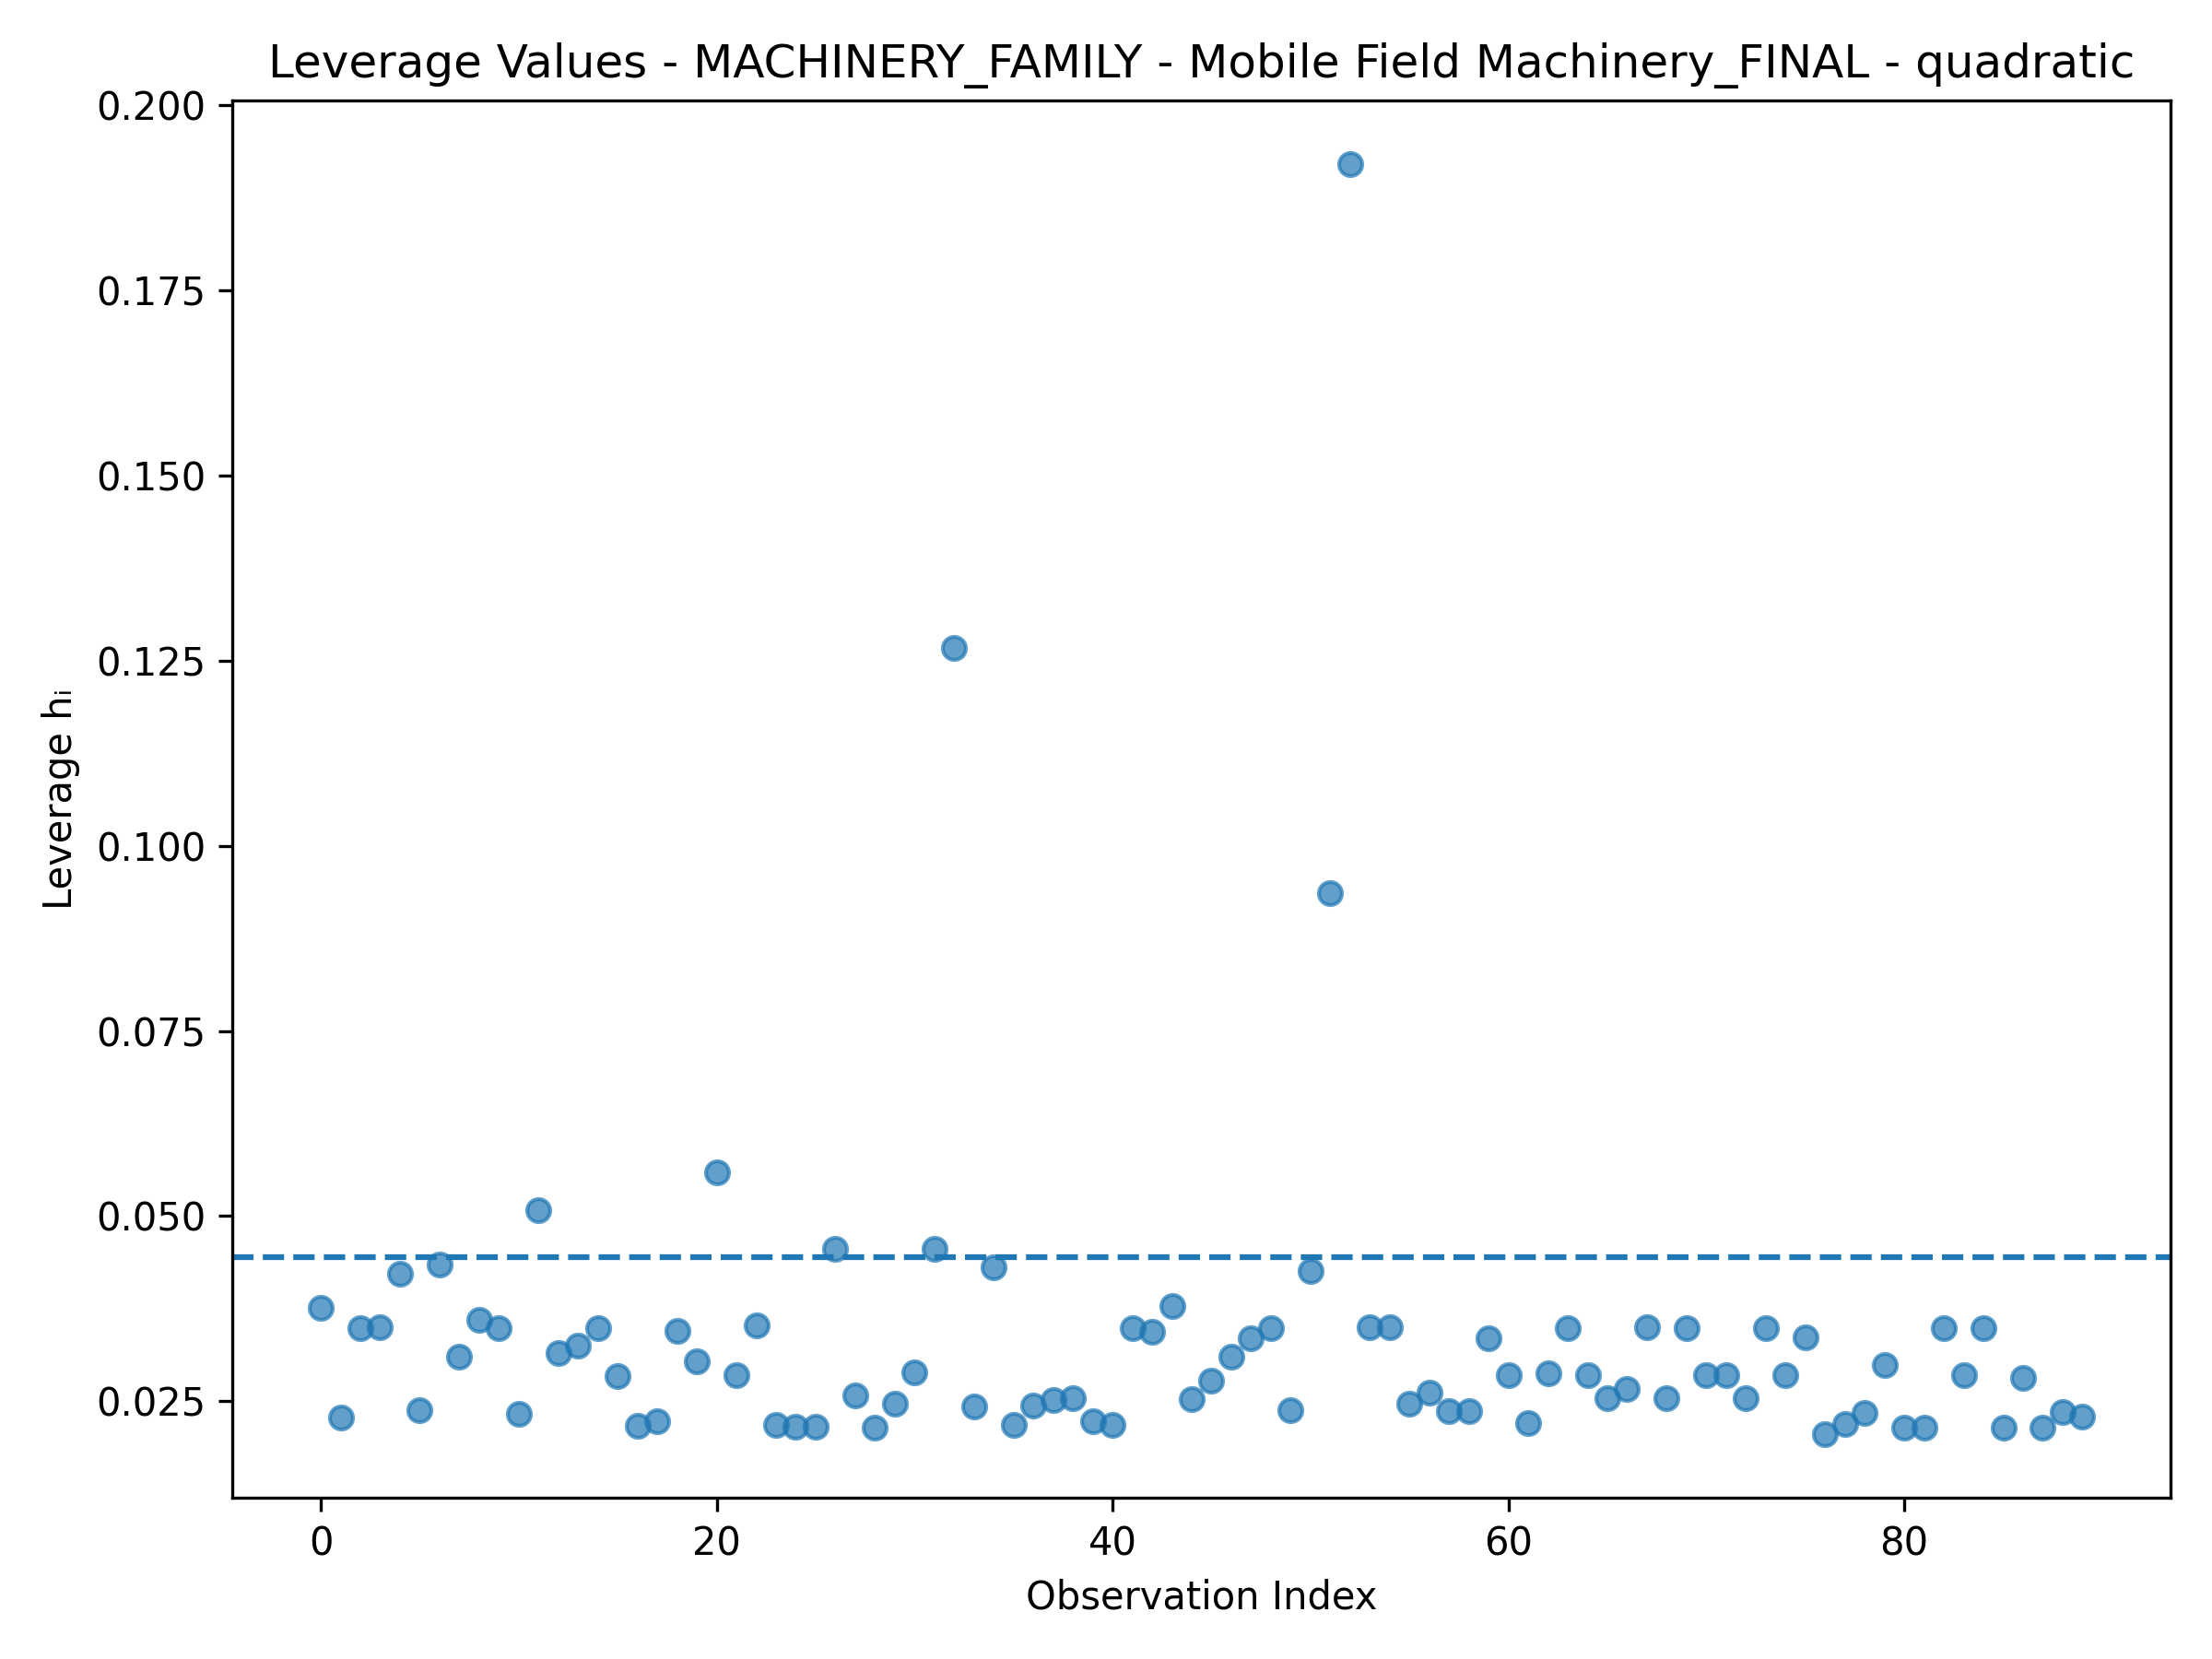
\includegraphics[width=0.48\linewidth]{MACHINERY_FAMILY_Mobile_Field_Machinery_FINAL_quadratic_leverage.png}
  \hfill
  
\includegraphics[width=0.48\linewidth]{MACHINERY_FAMILY_Mobile_Field_Machinery_FINAL_quadratic_studentized_residuals.png}
  \caption{Mobile Field Machinery --- leverage plot (left) and studentized residuals (right).}
\end{figure}

\subsection*{B.2 Machinery Family: Harvest Machinery}

\begin{figure}[H]
  \centering
  
\includegraphics[width=0.48\linewidth]{MACHINERY_FAMILY_Harvest_Machinery_FINAL_quadratic_residuals_vs_fitted.png}
  \hfill
  
\includegraphics[width=0.48\linewidth]{MACHINERY_FAMILY_Harvest_Machinery_FINAL_quadratic_qqplot.png}
  \caption{Harvest Machinery --- residuals vs.\ fitted (left) and Q-Q plot (right).}
\end{figure}

\begin{figure}[H]
  \centering
  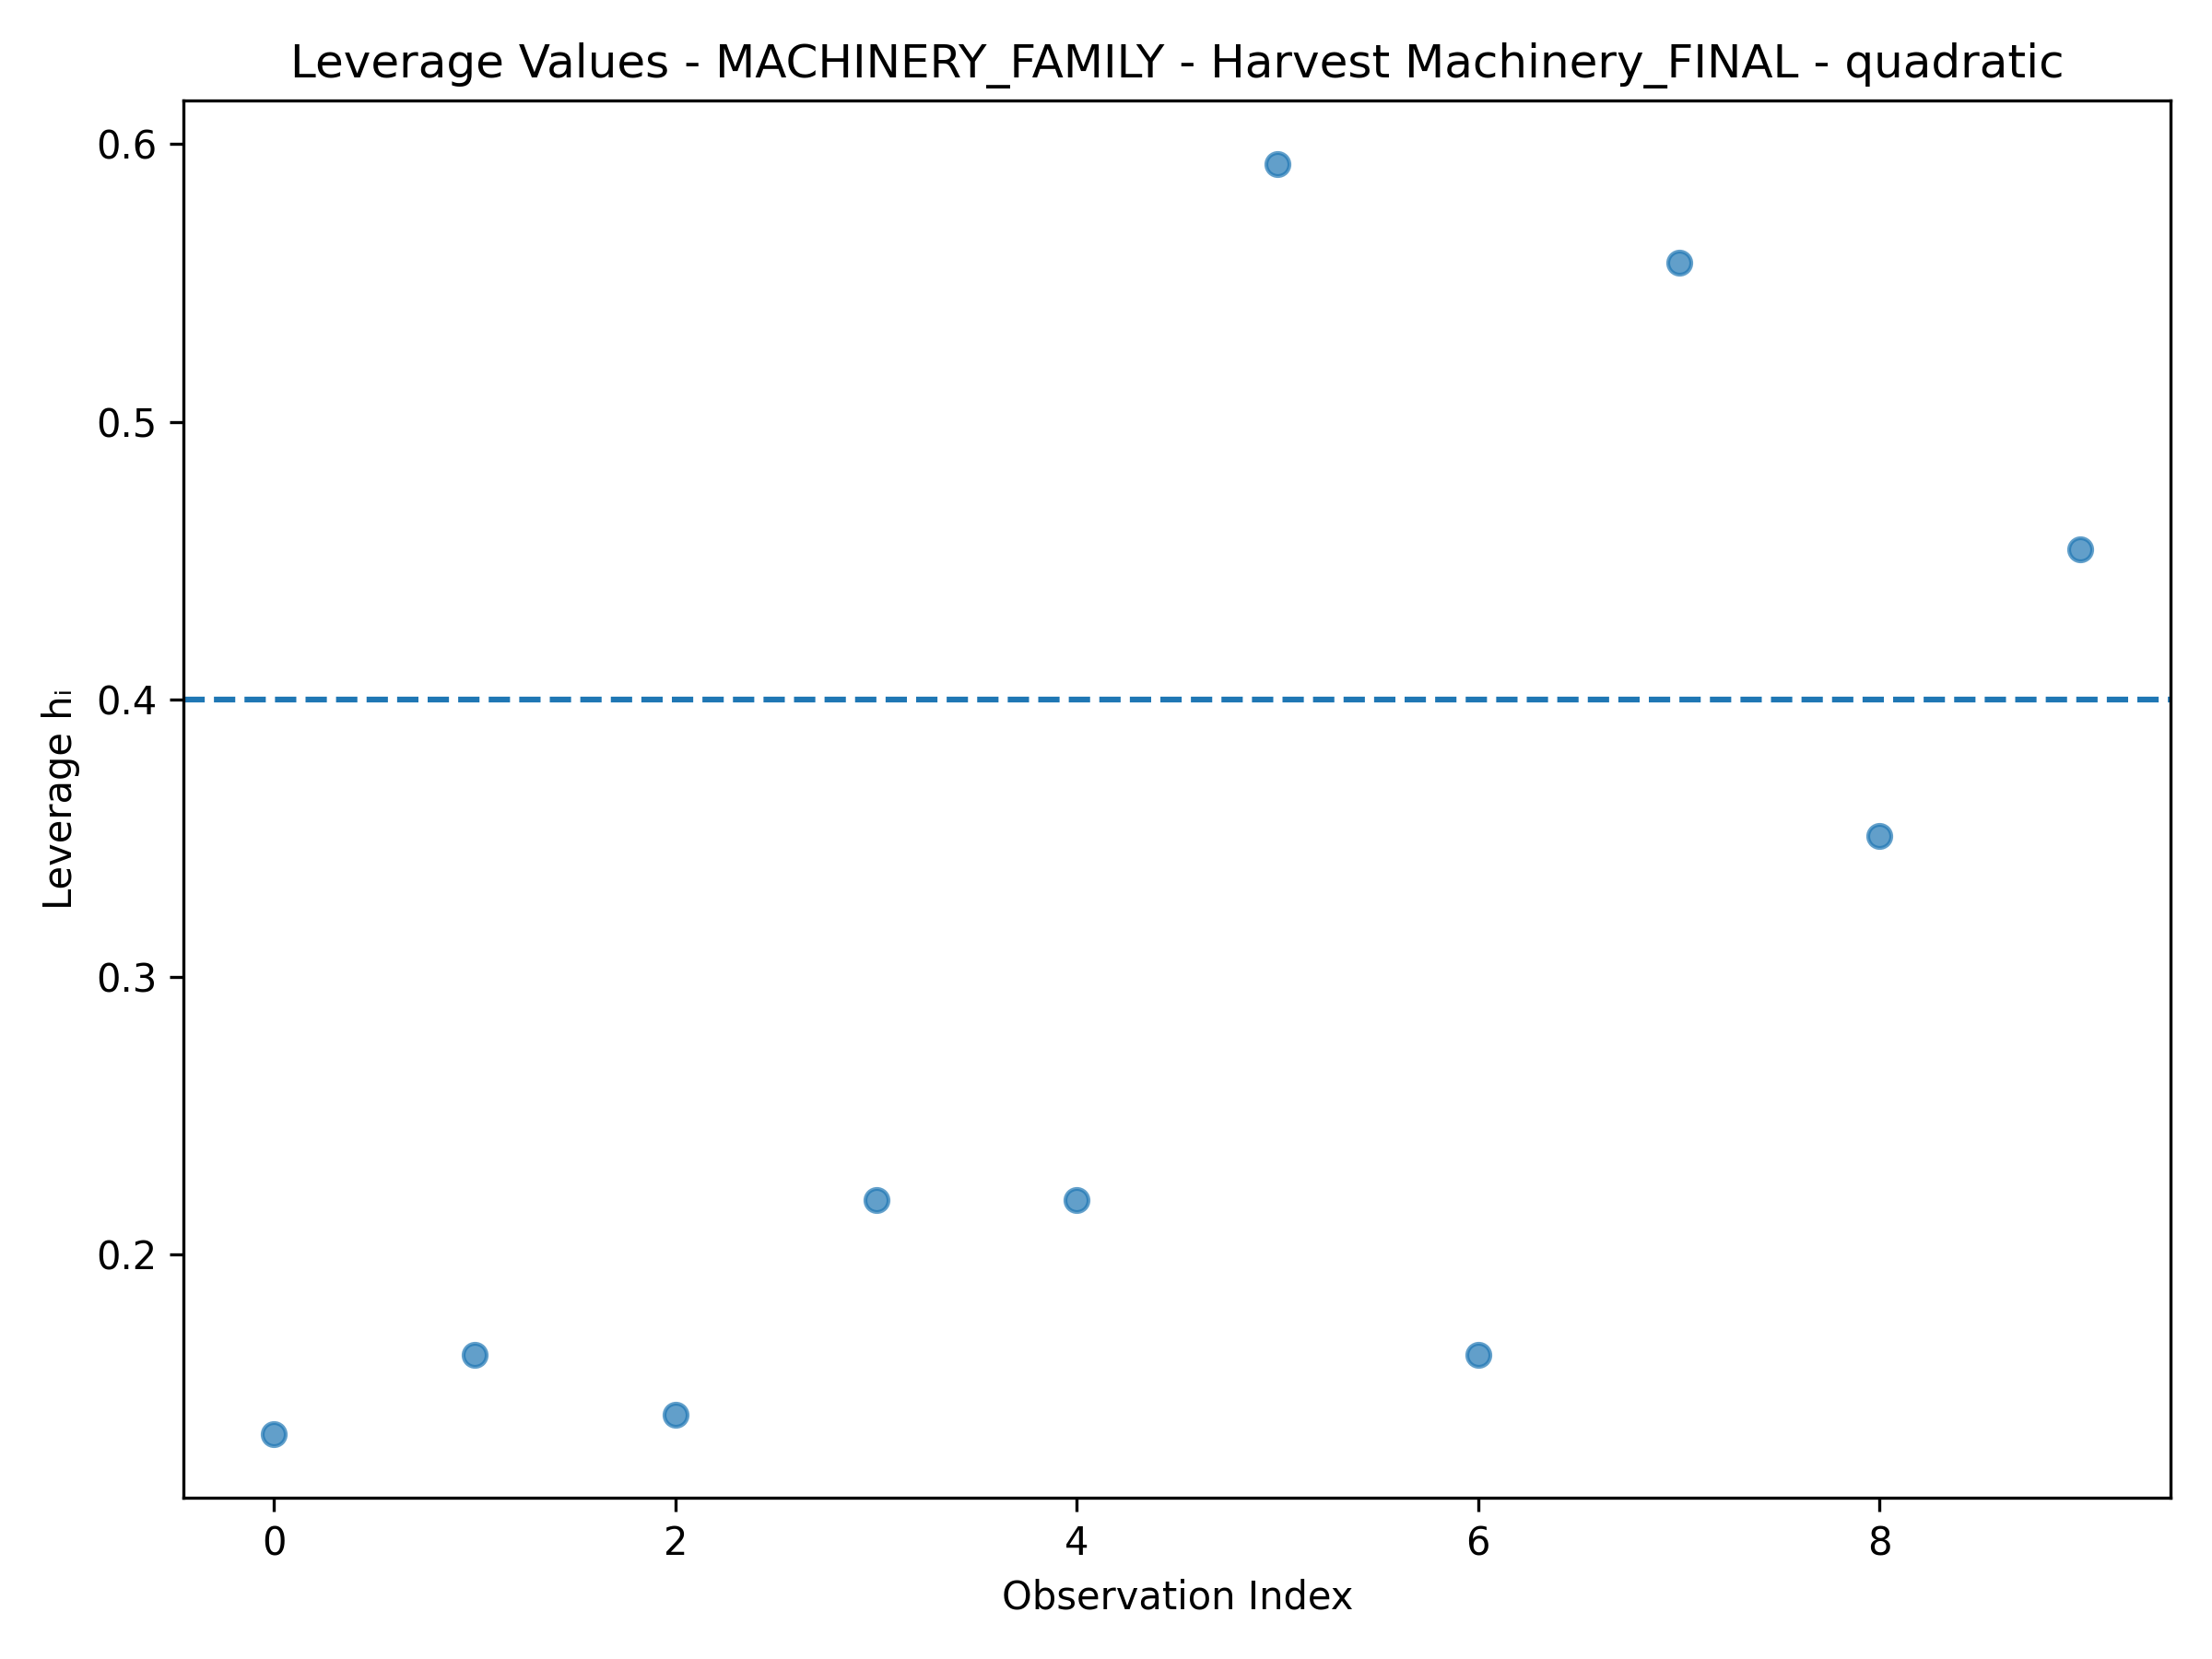
\includegraphics[width=0.48\linewidth]{MACHINERY_FAMILY_Harvest_Machinery_FINAL_quadratic_leverage.png}
  \hfill
  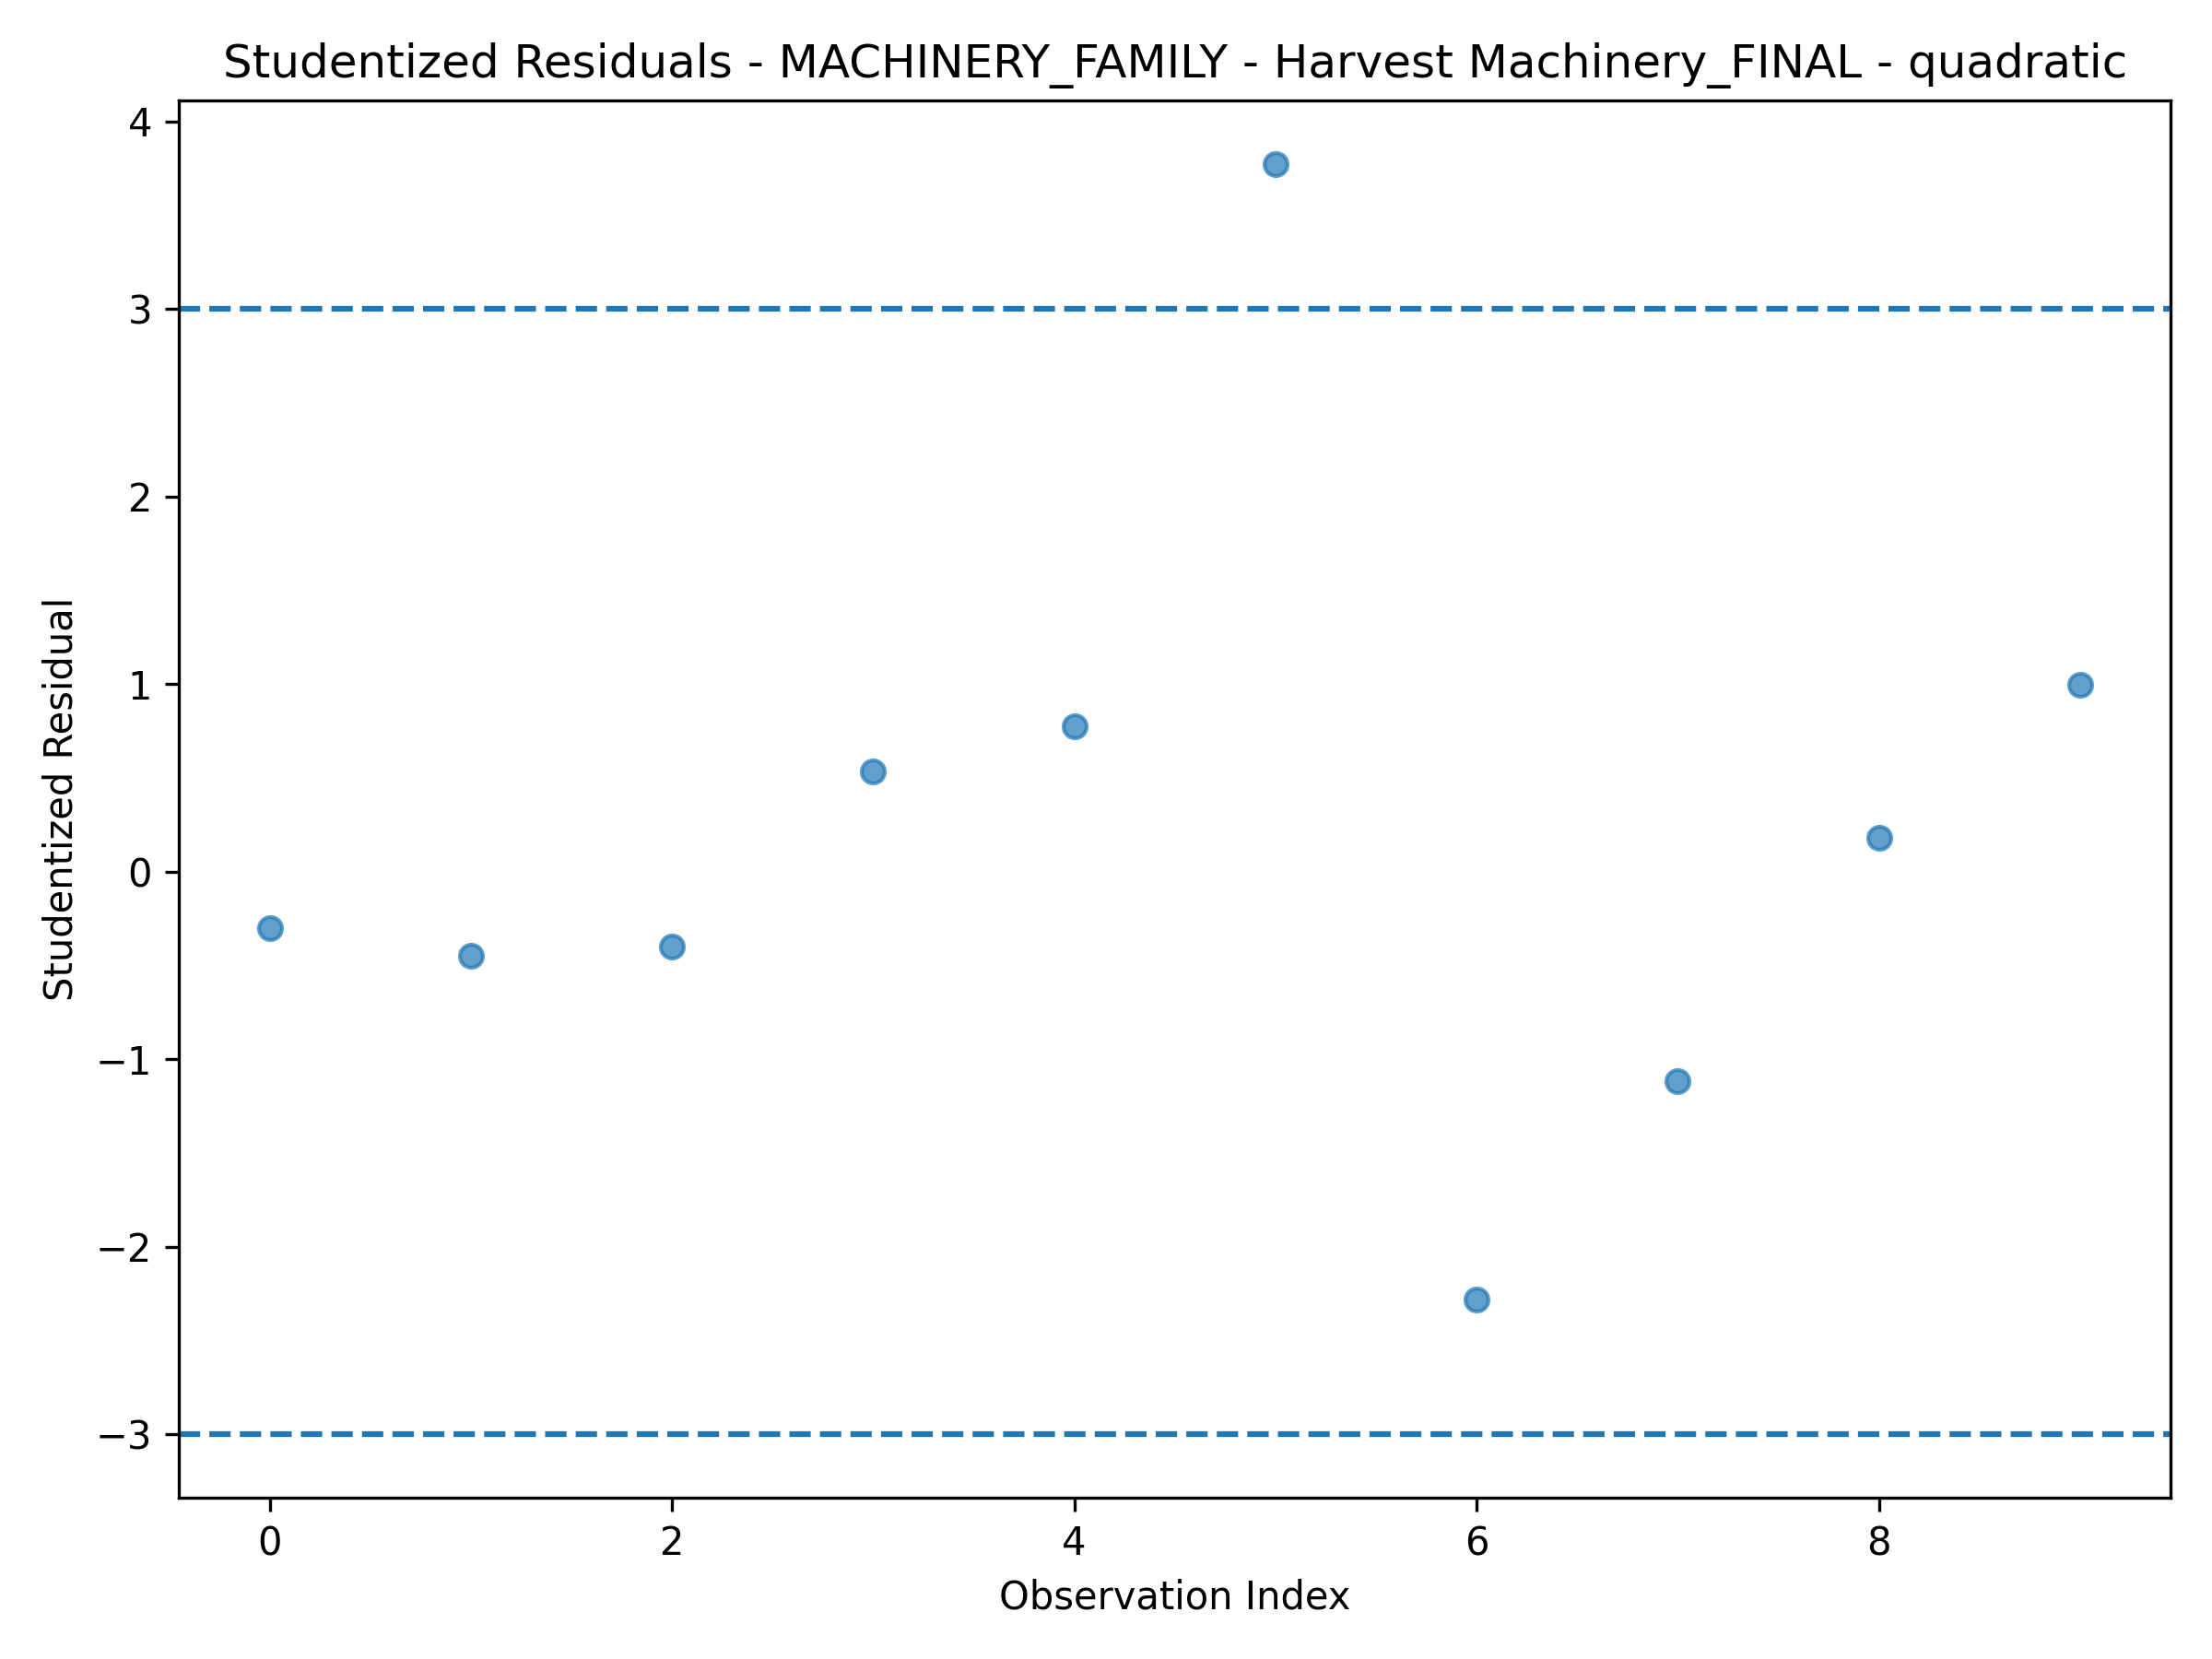
\includegraphics[width=0.48\linewidth]{MACHINERY_FAMILY_Harvest_Machinery_FINAL_quadratic_studentized_residuals.png}
  \caption{Harvest Machinery --- leverage plot (left) and studentized residuals (right).}
\end{figure}

\subsection*{B.3 Machinery Type: Four-Wheel Tractor}

\begin{figure}[H]
  \centering
  
\includegraphics[width=0.48\linewidth]{MACHINERY_TYPE_Four_Wheel_Tractor_FINAL_quadratic_residuals_vs_fitted.png}
  \hfill
  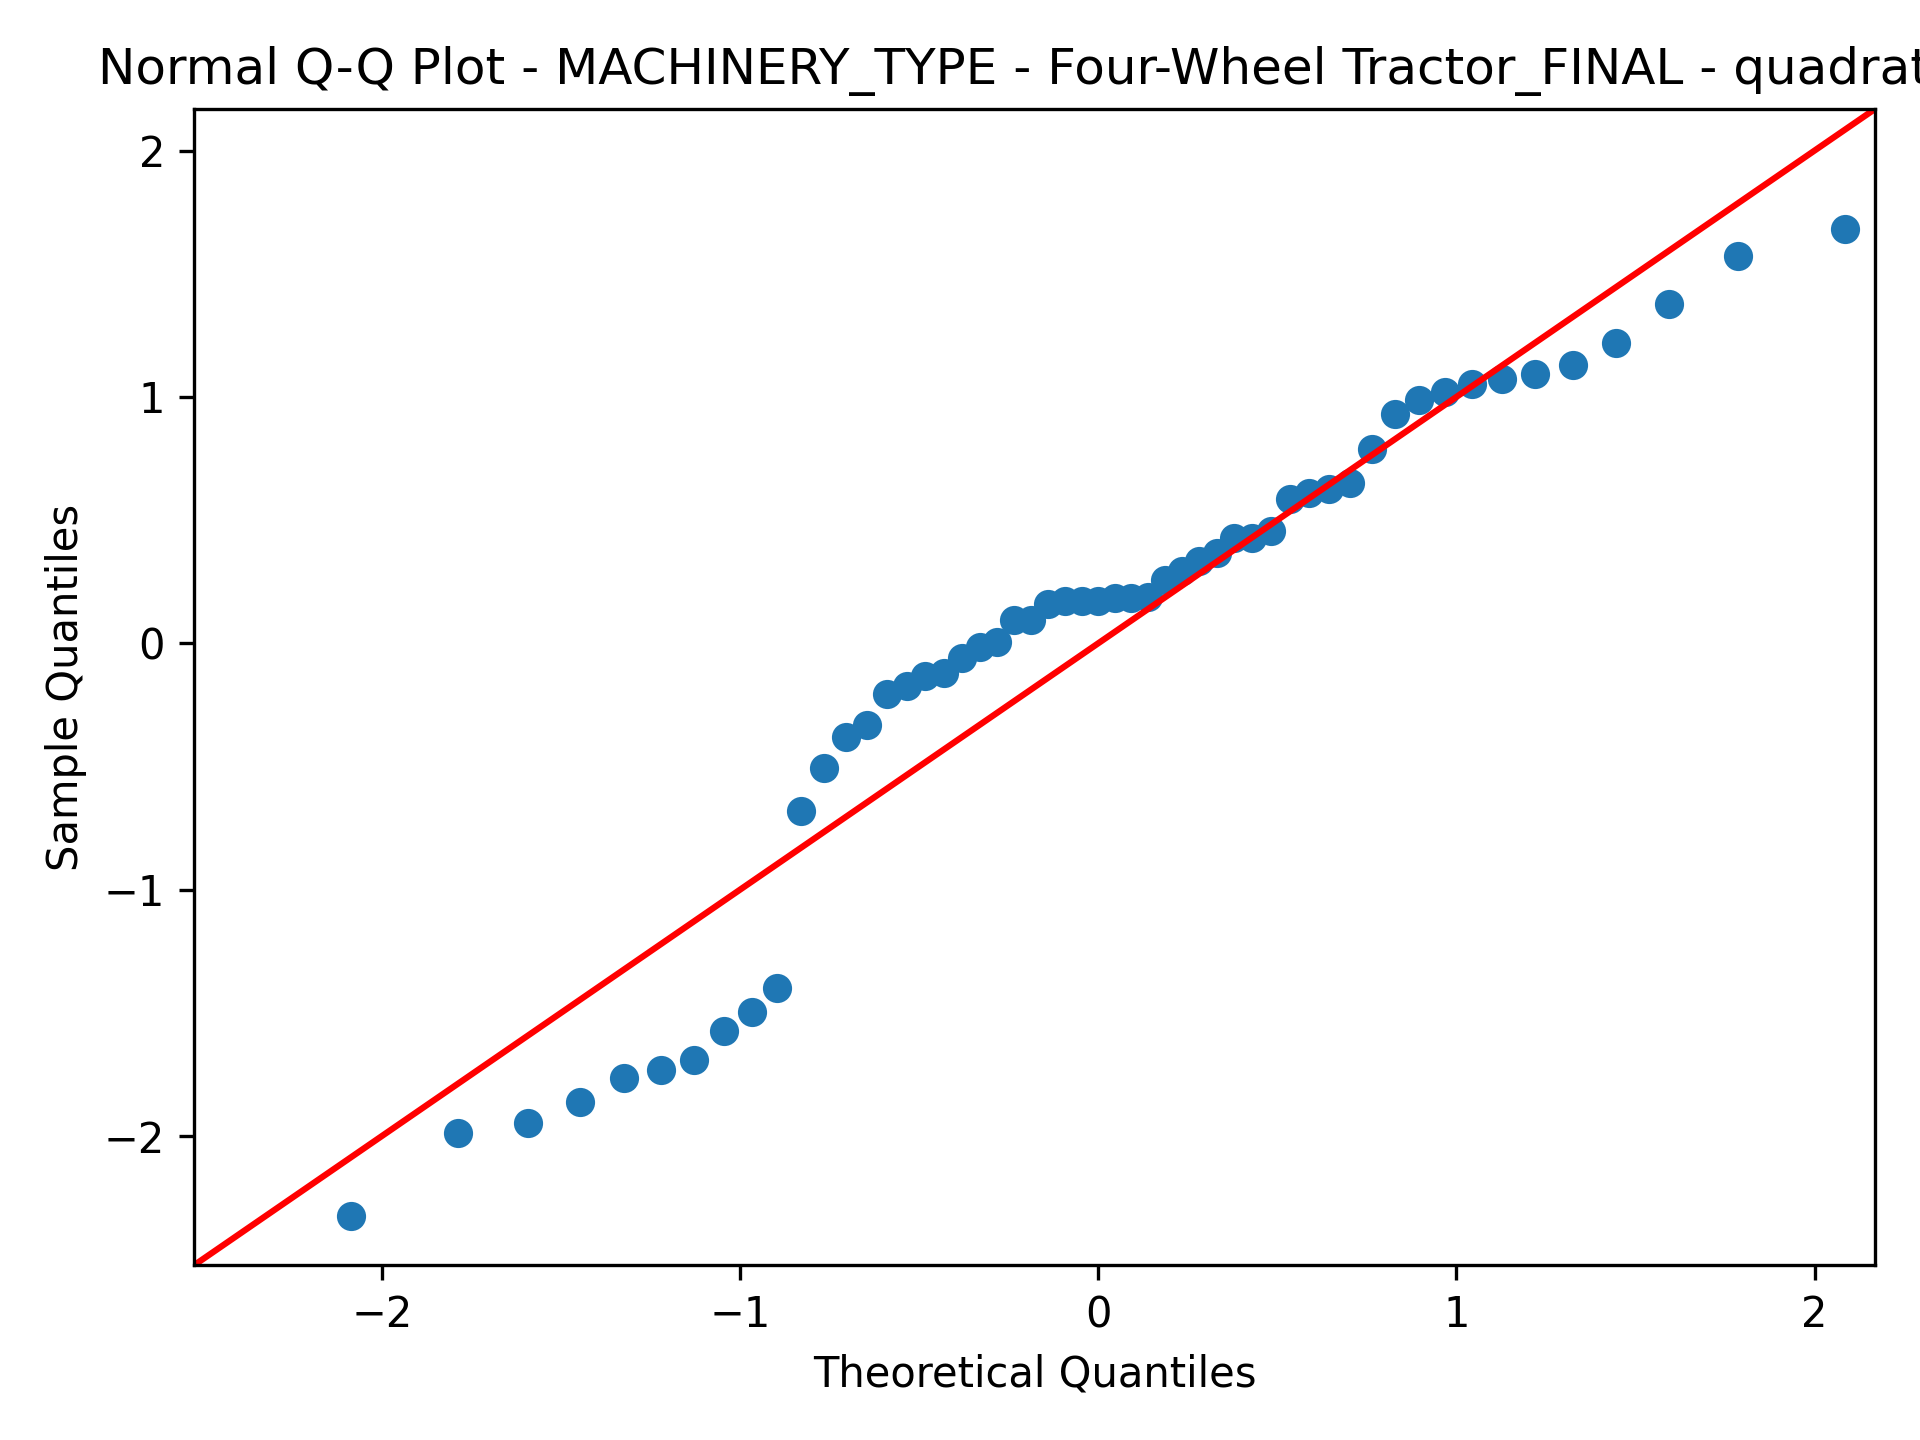
\includegraphics[width=0.48\linewidth]{MACHINERY_TYPE_Four_Wheel_Tractor_FINAL_quadratic_qqplot.png}
  \caption{Four-Wheel Tractor --- residuals vs.\ fitted (left) and Q-Q plot (right).}
\end{figure}

\begin{figure}[H]
  \centering
  
\includegraphics[width=0.48\linewidth]{MACHINERY_TYPE_Four_Wheel_Tractor_FINAL_quadratic_leverage.png}
  \hfill
  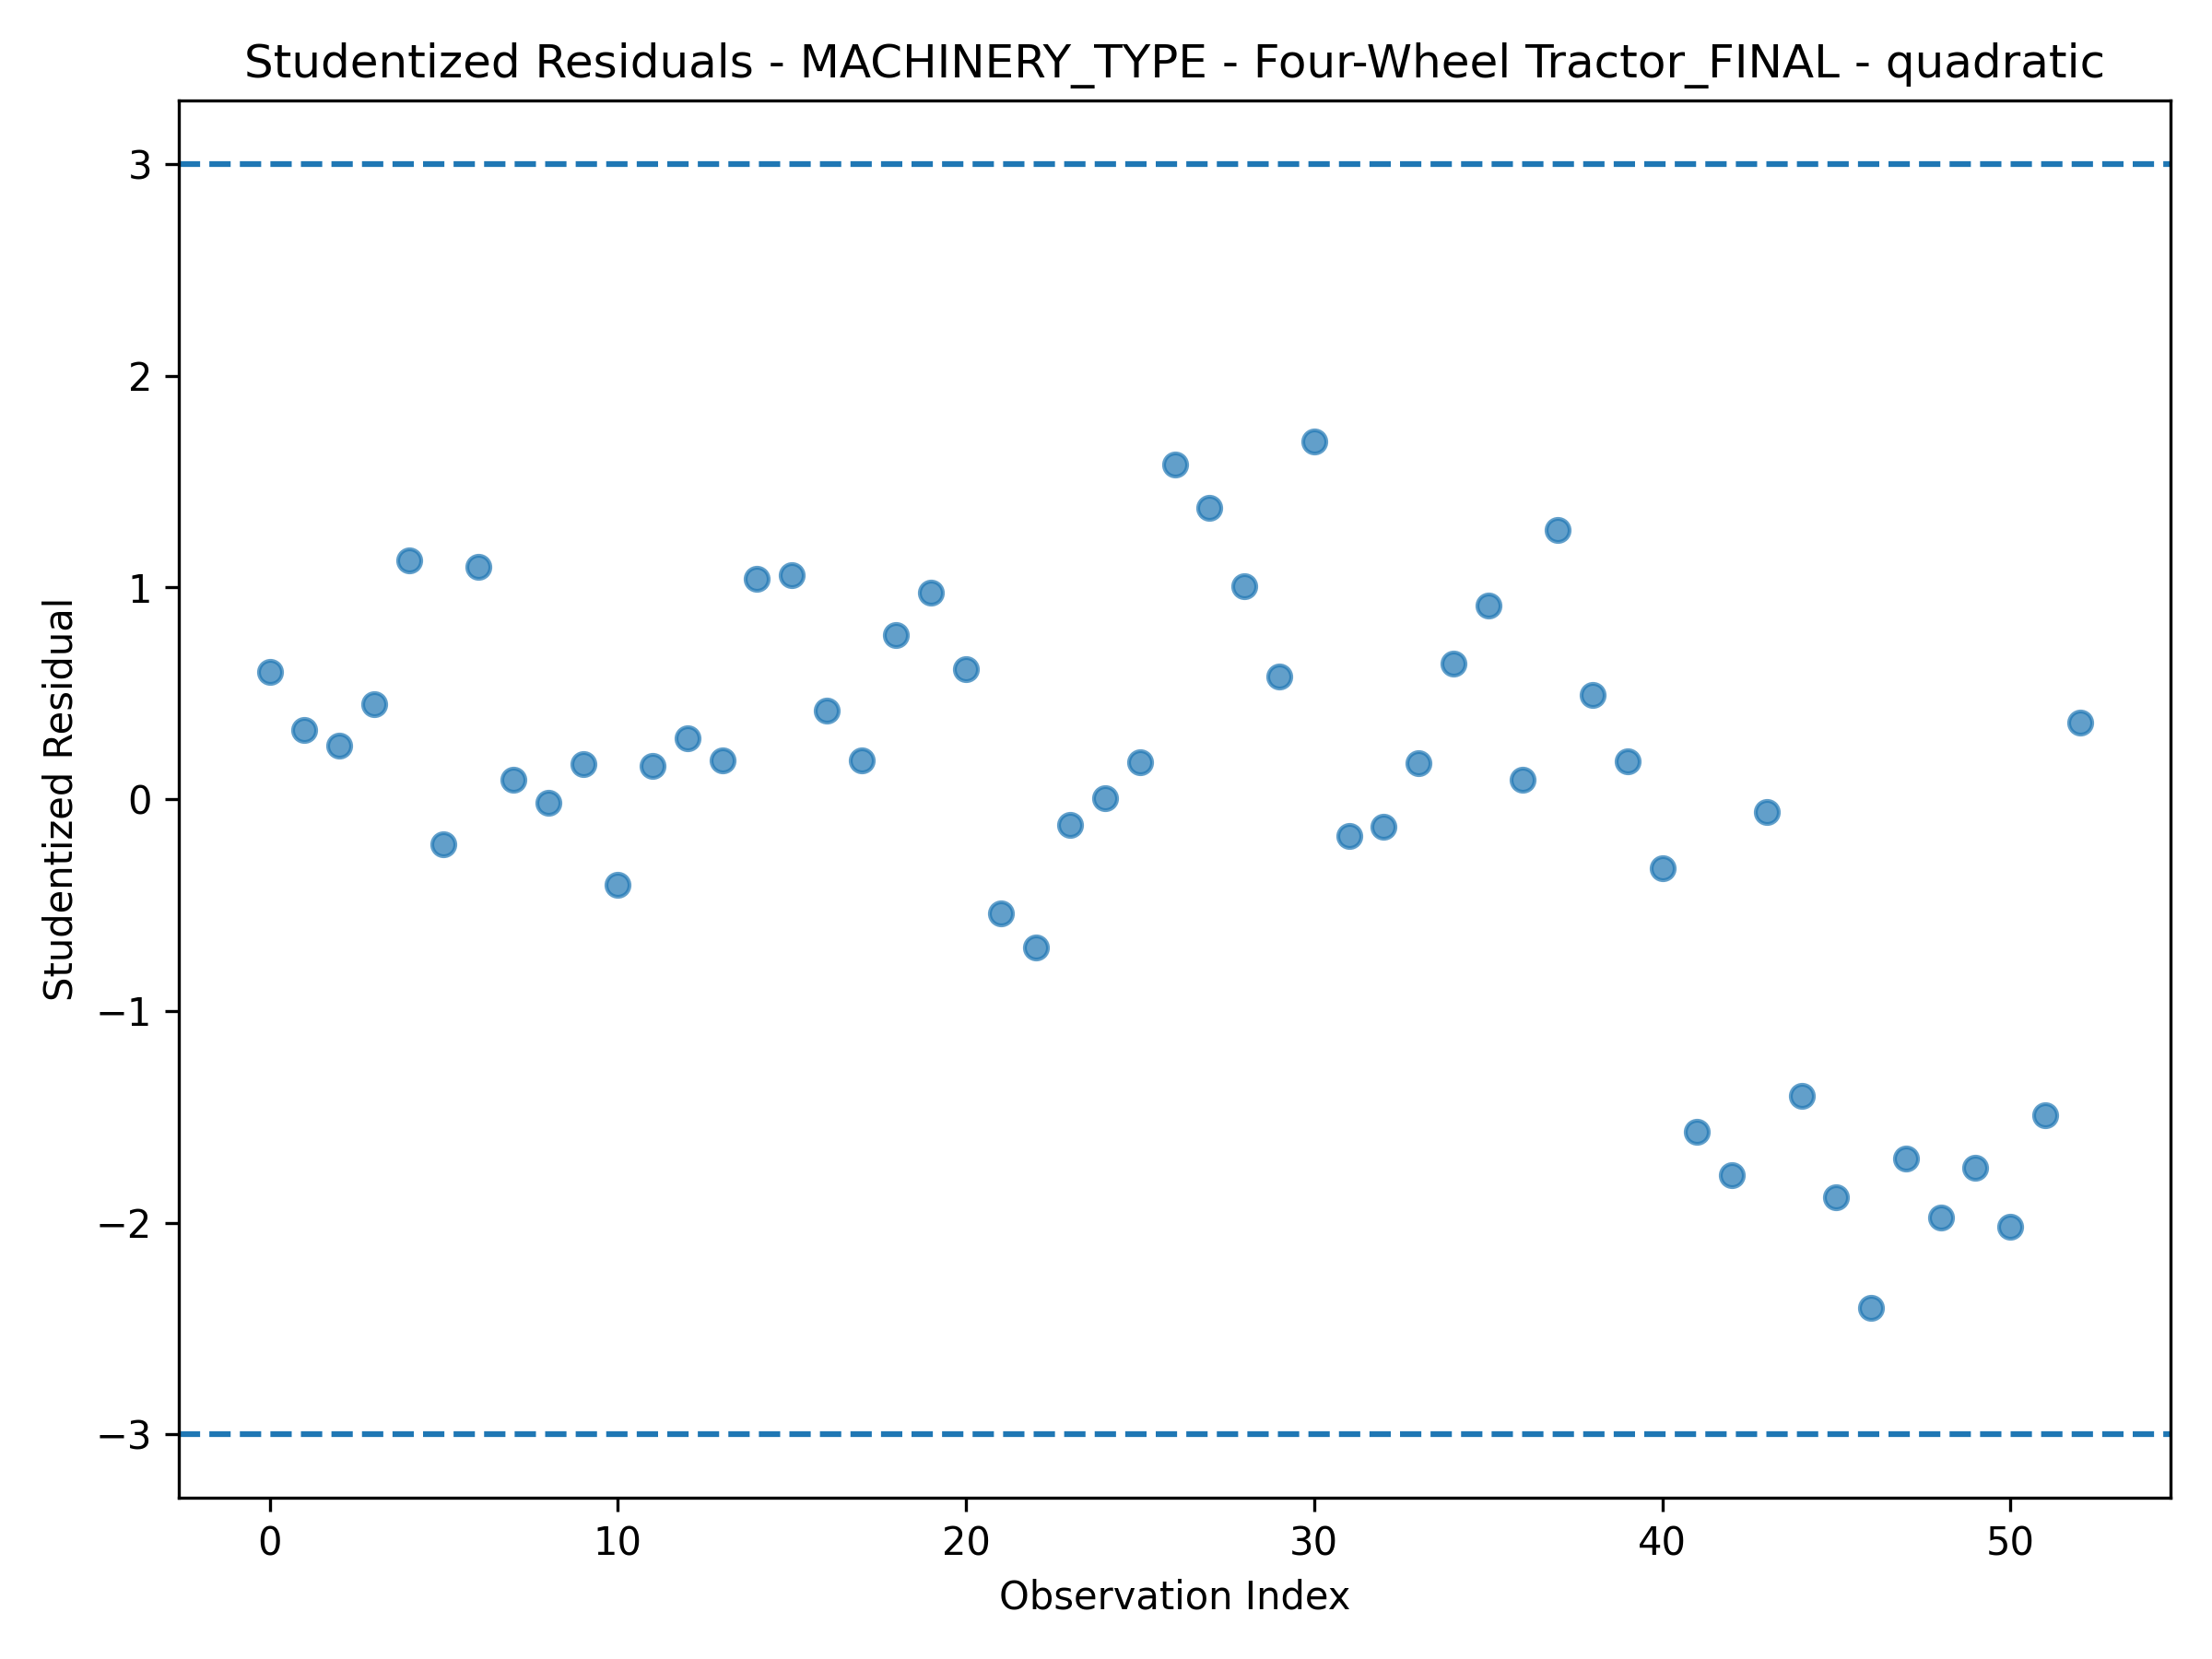
\includegraphics[width=0.48\linewidth]{MACHINERY_TYPE_Four_Wheel_Tractor_FINAL_quadratic_studentized_residuals.png}
  \caption{Four-Wheel Tractor --- leverage plot (left) and studentized residuals (right).}
\end{figure}

\subsection*{B.4 Machinery Type: Combine Harvester}

\begin{figure}[H]
  \centering
  
\includegraphics[width=0.48\linewidth]{MACHINERY_TYPE_Combine_Harvester_FINAL_quadratic_residuals_vs_fitted.png}
  \hfill
  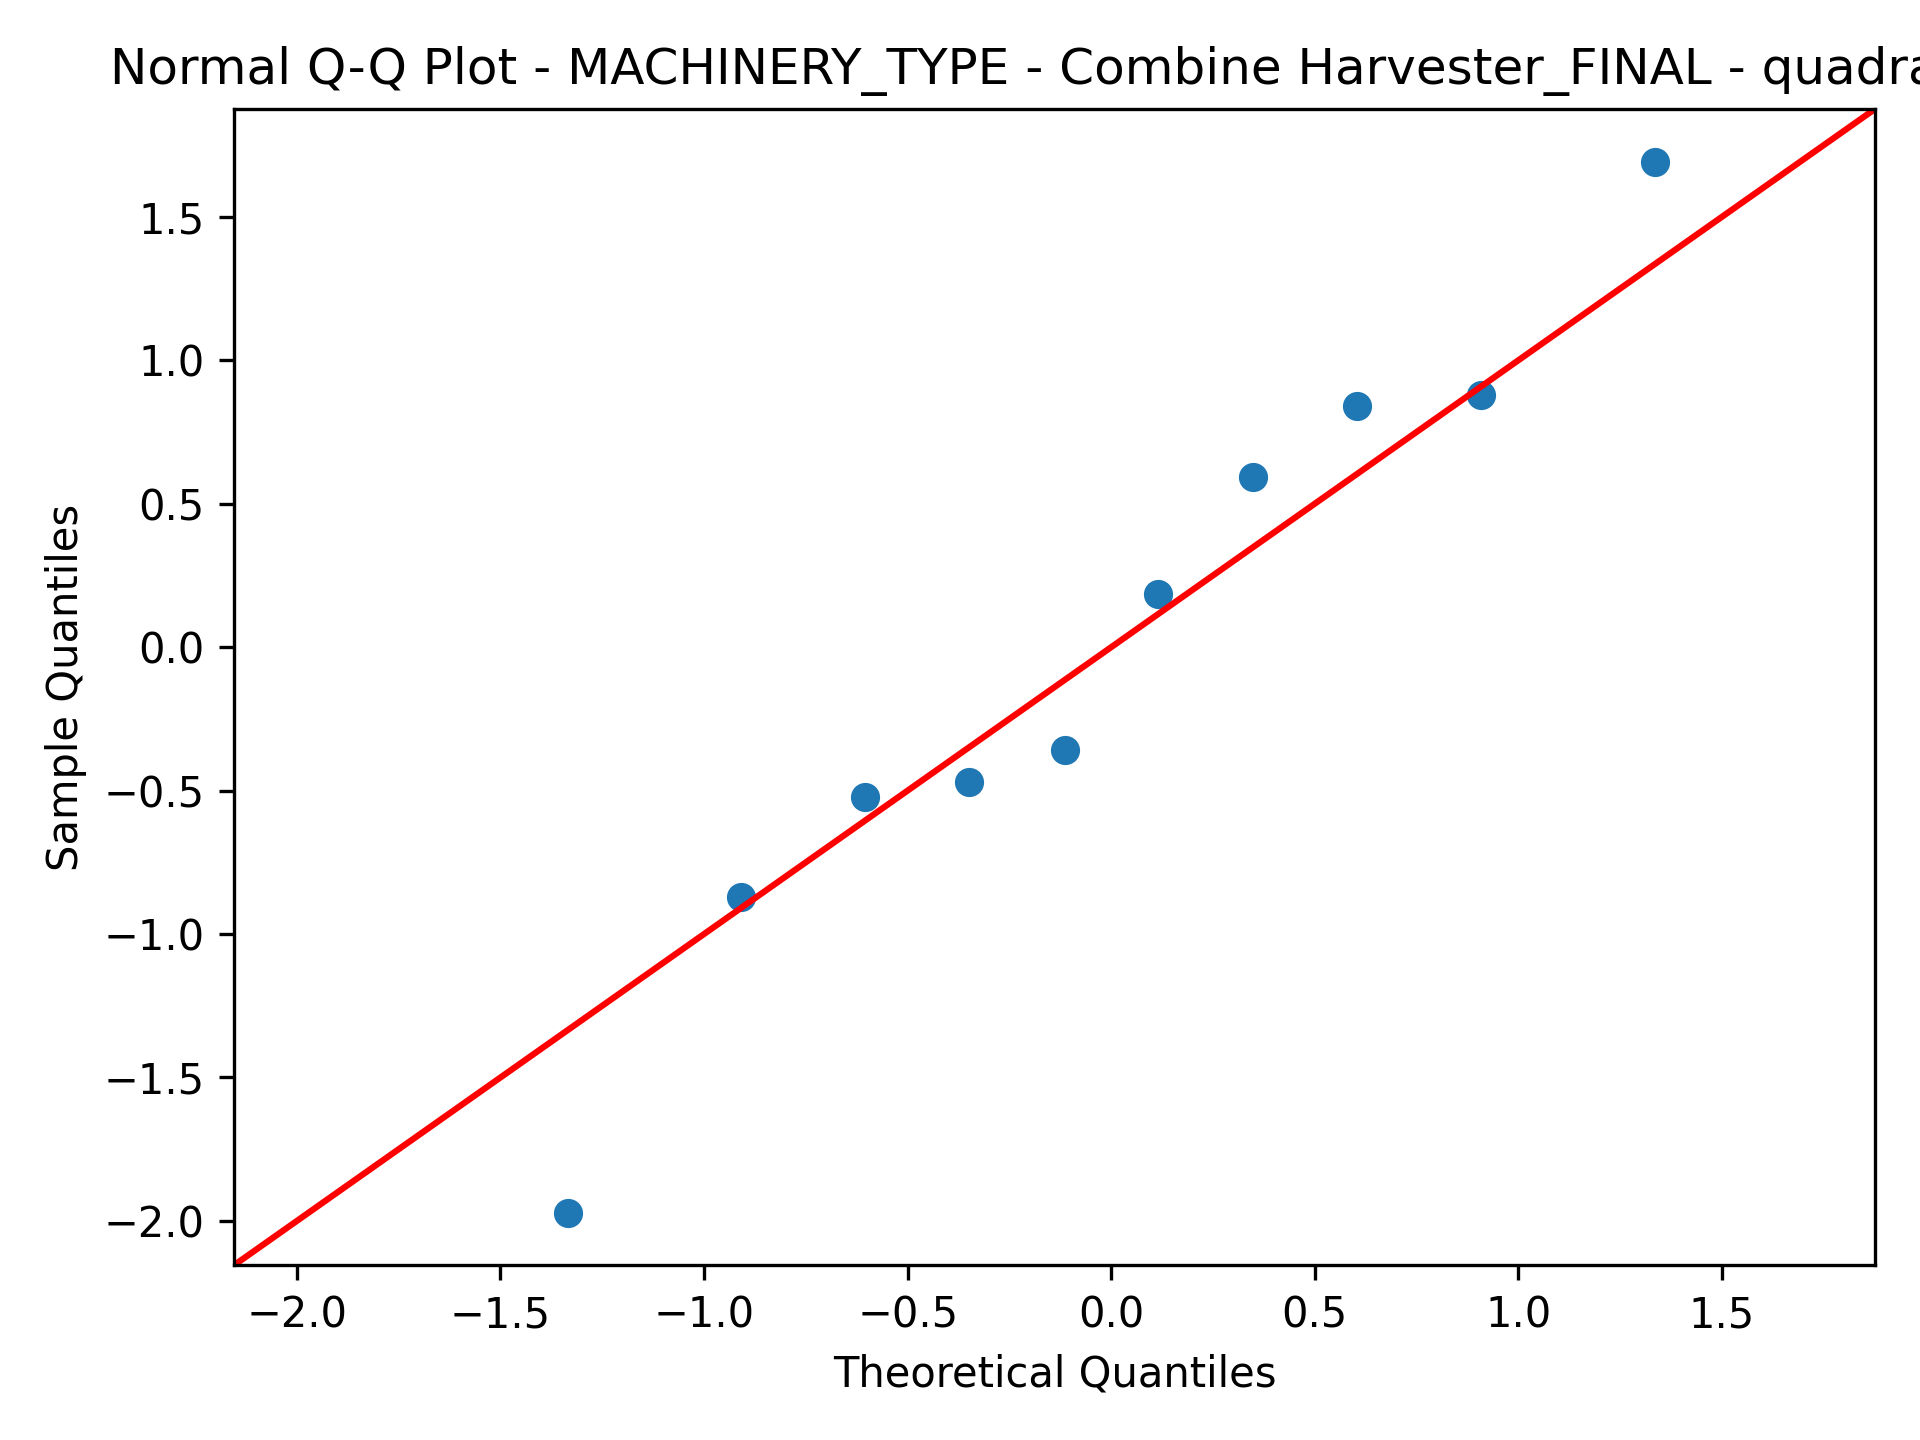
\includegraphics[width=0.48\linewidth]{MACHINERY_TYPE_Combine_Harvester_FINAL_quadratic_qqplot.png}
  \caption{Combine Harvester --- residuals vs.\ fitted (left) and Q-Q plot (right).}
\end{figure}

\begin{figure}[H]
  \centering
  
\includegraphics[width=0.48\linewidth]{MACHINERY_TYPE_Combine_Harvester_FINAL_quadratic_leverage.png}
  \hfill
  
\includegraphics[width=0.48\linewidth]{MACHINERY_TYPE_Combine_Harvester_FINAL_quadratic_studentized_residuals.png}
  \caption{Combine Harvester --- leverage plot (left) and studentized residuals (right).}
\end{figure}

\subsection*{B.5 Machinery Type: Mechanical Dryer}

\begin{figure}[H]
  \centering
  
\includegraphics[width=0.48\linewidth]{MACHINERY_TYPE_Mechanical_Dryer_FINAL_quadratic_residuals_vs_fitted.png}
  \hfill
  
\includegraphics[width=0.48\linewidth]{MACHINERY_TYPE_Mechanical_Dryer_FINAL_quadratic_qqplot.png}
  \caption{Mechanical Dryer --- residuals vs.\ fitted (left) and Q-Q plot (right).}
\end{figure}

\begin{figure}[H]
  \centering
  
\includegraphics[width=0.48\linewidth]{MACHINERY_TYPE_Mechanical_Dryer_FINAL_quadratic_leverage.png}
  \hfill
  
\includegraphics[width=0.48\linewidth]{MACHINERY_TYPE_Mechanical_Dryer_FINAL_quadratic_studentized_residuals.png}
  \caption{Mechanical Dryer --- leverage plot (left) and studentized residuals (right).}
\end{figure}

\subsection*{B.6 Global Model: All Machinery}

\begin{figure}[H]
  \centering
  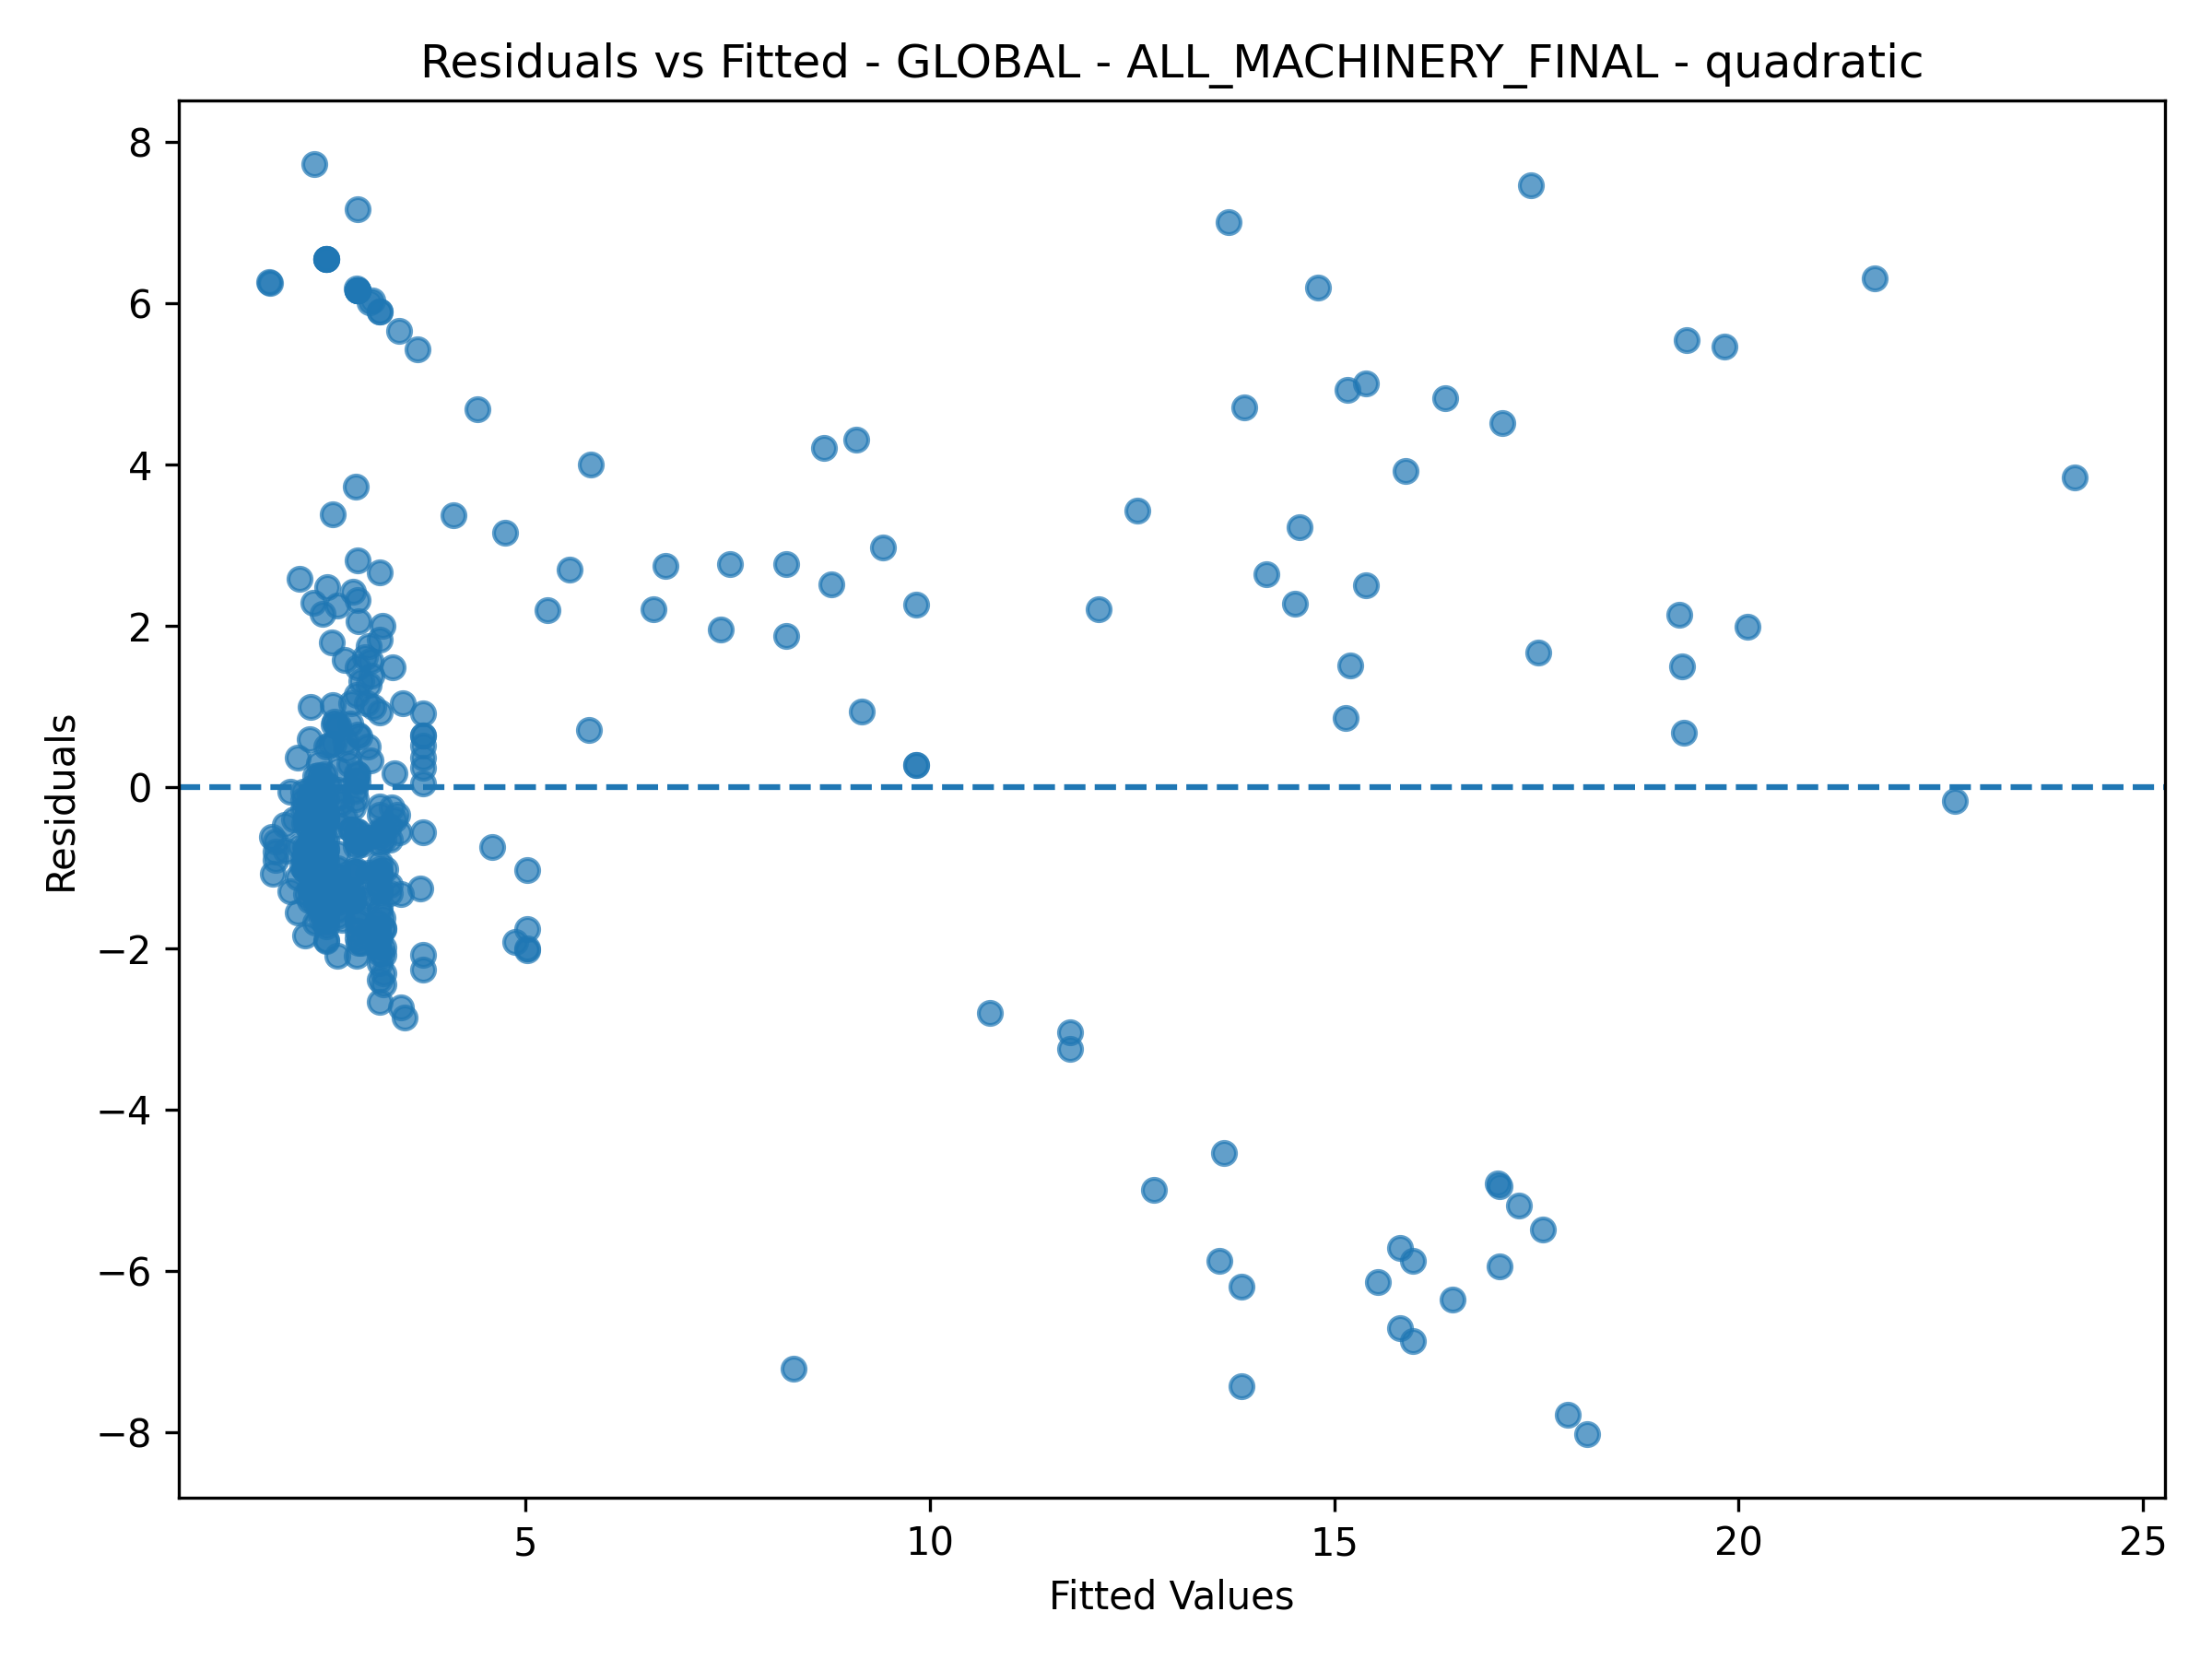
\includegraphics[width=0.48\linewidth]{GLOBAL_ALL_MACHINERY_FINAL_quadratic_residuals_vs_fitted.png}
  \hfill
  
\includegraphics[width=0.48\linewidth]{GLOBAL_ALL_MACHINERY_FINAL_quadratic_qqplot.png}
  \caption{Global (All Machinery) --- residuals vs.\ fitted (left) and Q-Q plot (right).}
\end{figure}

\begin{figure}[H]
  \centering
  
\includegraphics[width=0.48\linewidth]{GLOBAL_ALL_MACHINERY_FINAL_quadratic_leverage.png}
  \hfill
  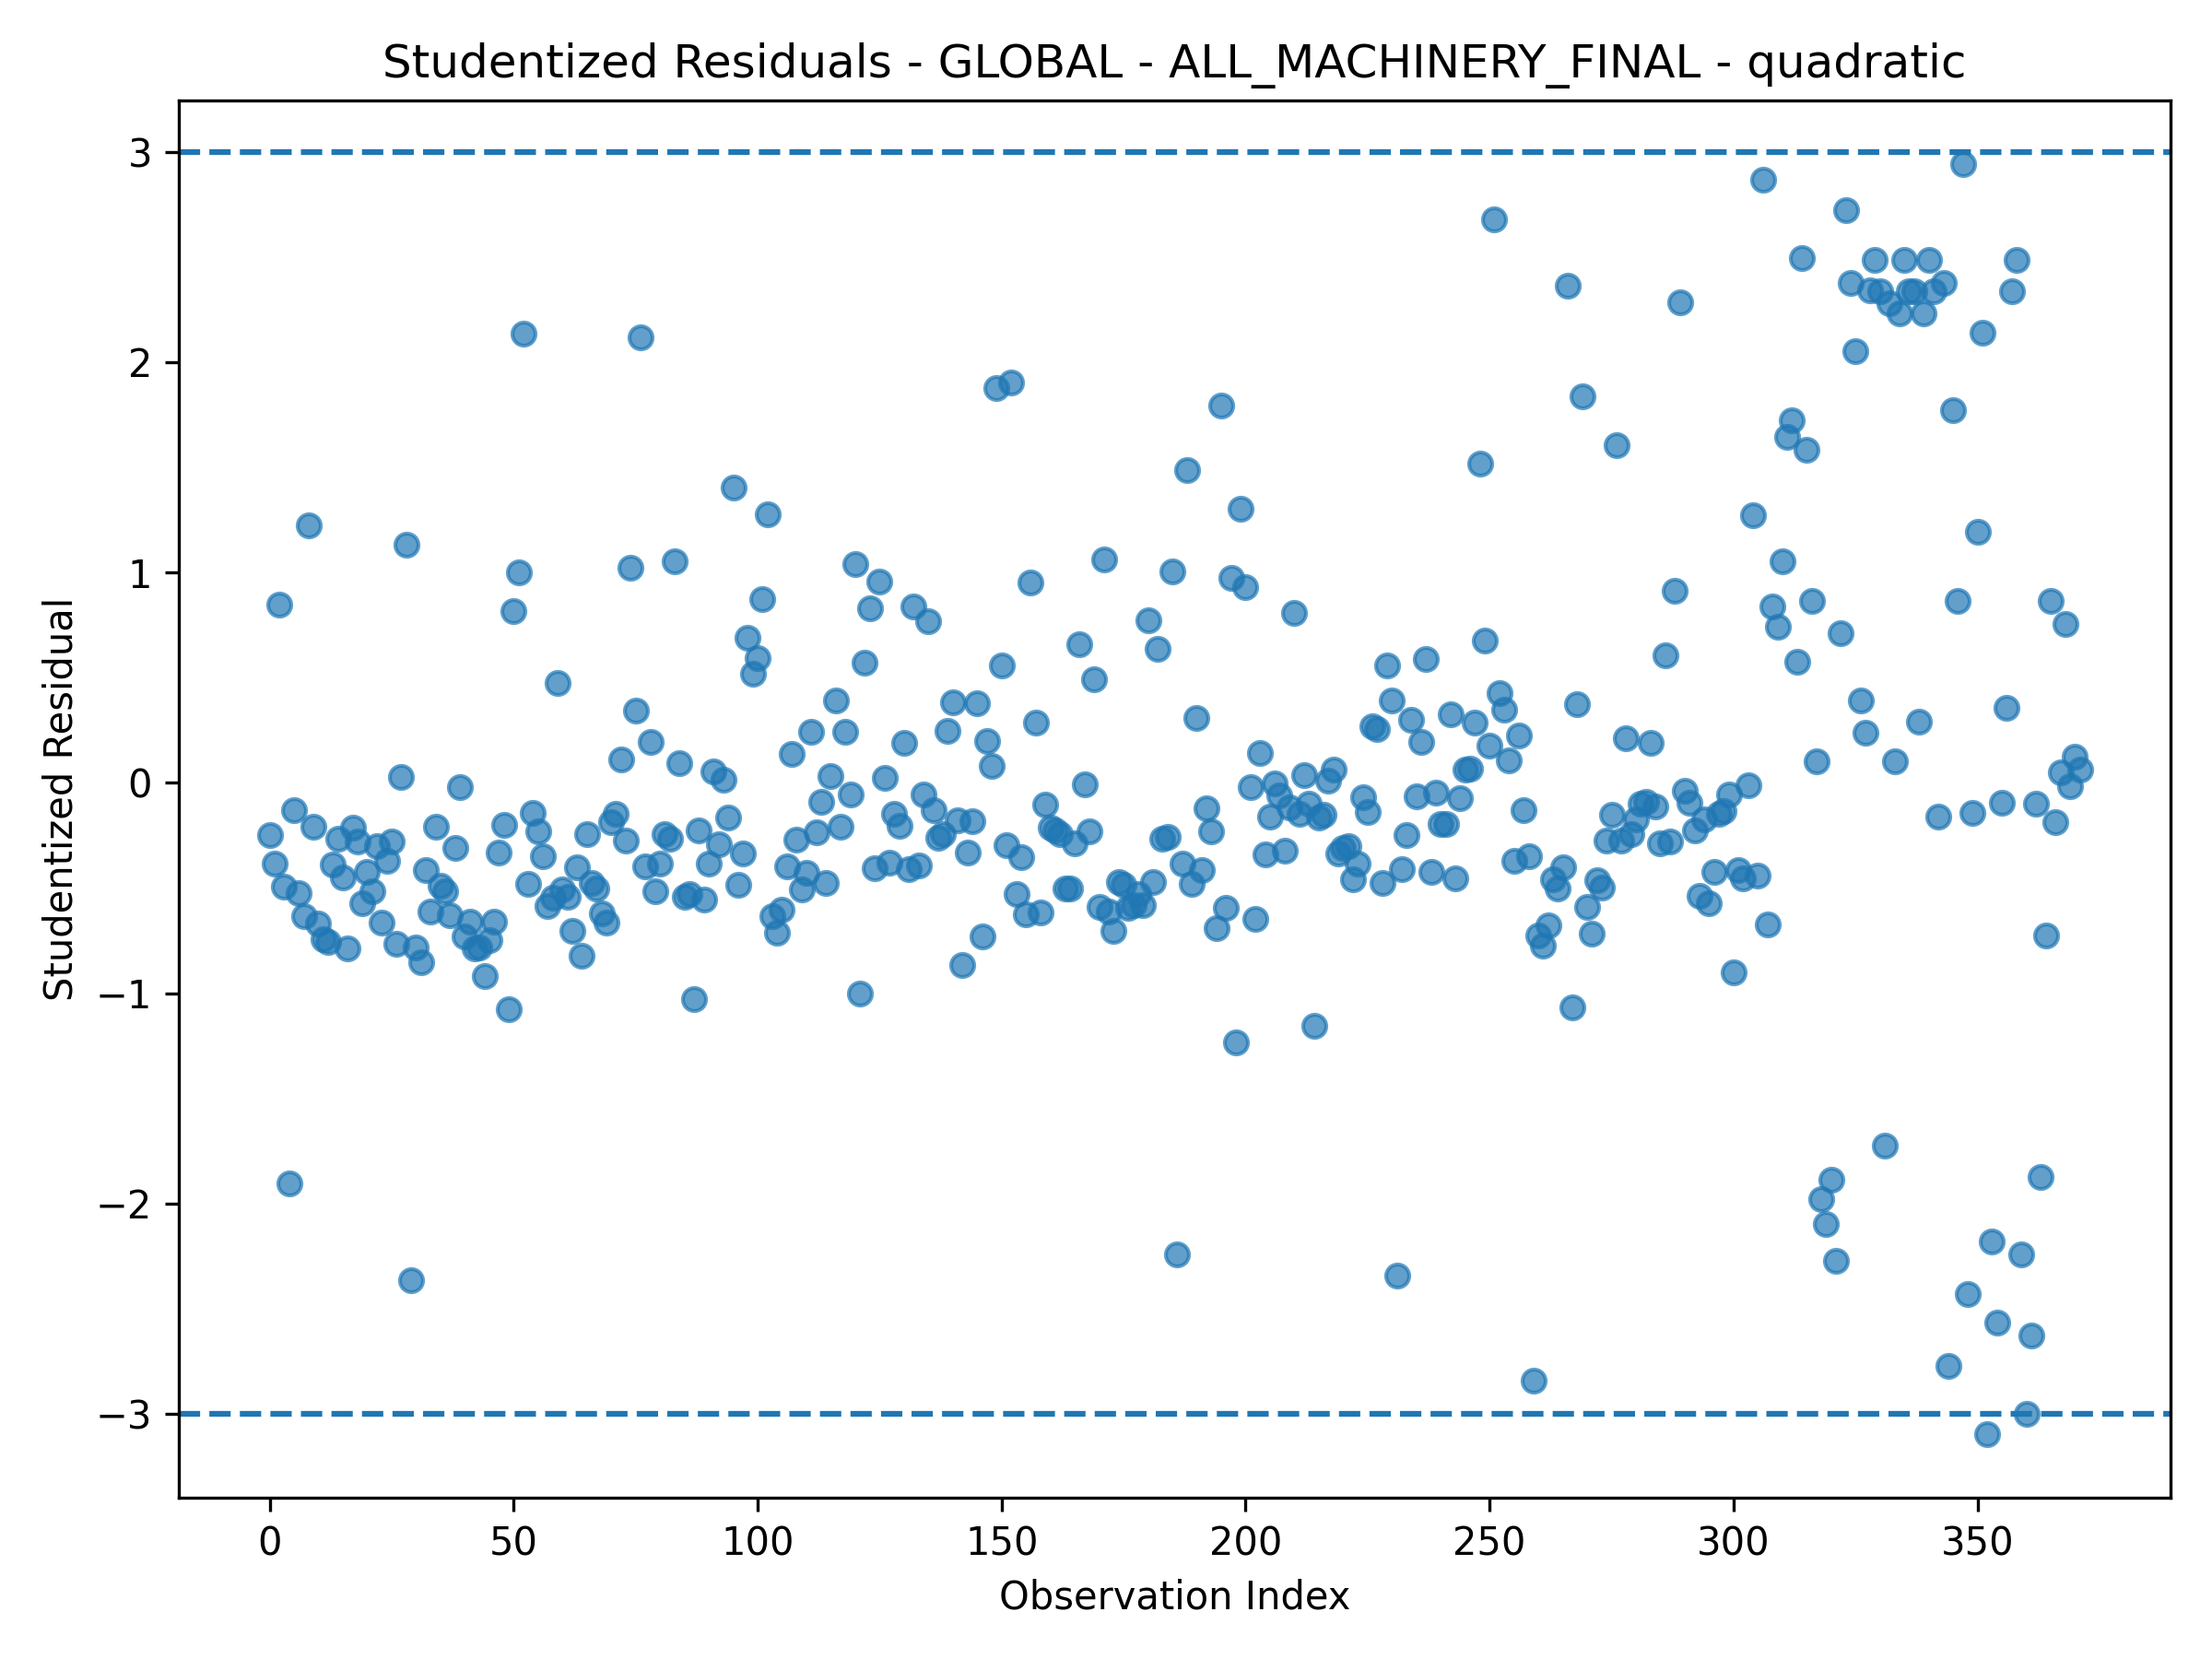
\includegraphics[width=0.48\linewidth]{GLOBAL_ALL_MACHINERY_FINAL_quadratic_studentized_residuals.png}
  \caption{Global (All Machinery) --- leverage plot (left) and studentized residuals (right).}
\end{figure}

%% ─────────────────────────────────────────────────────────────────────────────
\section*{Appendix C: LIME Local Explanations}

LIME tabular explainer was applied to 10 representative records from the test set. Each figure shows the local feature contributions for one record, with green bars indicating features that increased the predicted fuel consumption and red bars indicating features that decreased it.

\begin{figure}[H]
  \centering
  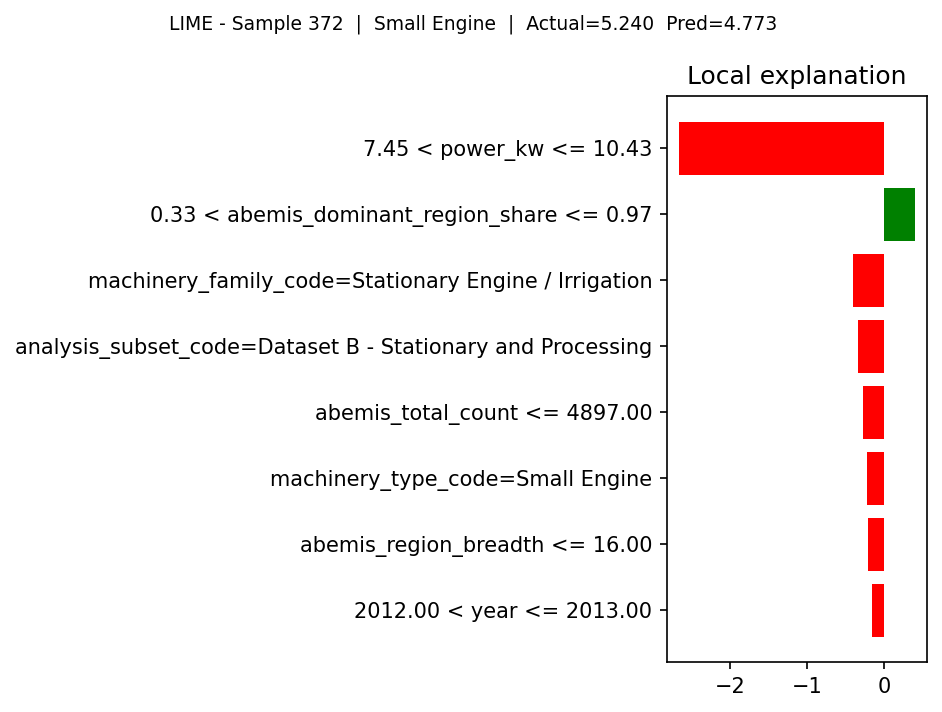
\includegraphics[width=0.85\linewidth]{lime_example_0.png}
  \caption{LIME local explanation --- example record 0.}
\end{figure}

\begin{figure}[H]
  \centering
  
\includegraphics[width=0.85\linewidth]{lime_example_1.png}
  \caption{LIME local explanation --- example record 1.}
\end{figure}

\begin{figure}[H]
  \centering
  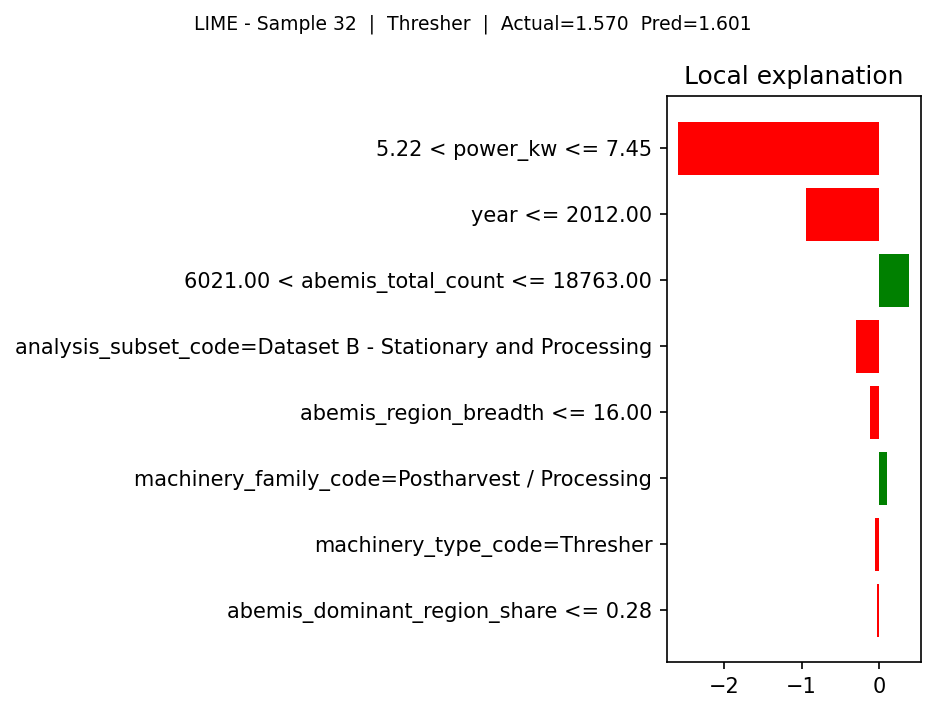
\includegraphics[width=0.85\linewidth]{lime_example_2.png}
  \caption{LIME local explanation --- example record 2.}
\end{figure}

\begin{figure}[H]
  \centering
  
\includegraphics[width=0.85\linewidth]{lime_example_3.png}
  \caption{LIME local explanation --- example record 3.}
\end{figure}

\begin{figure}[H]
  \centering
  
\includegraphics[width=0.85\linewidth]{lime_example_4.png}
  \caption{LIME local explanation --- example record 4.}
\end{figure}

\begin{figure}[H]
  \centering
  
\includegraphics[width=0.85\linewidth]{lime_example_5.png}
  \caption{LIME local explanation --- example record 5.}
\end{figure}

\begin{figure}[H]
  \centering
  
\includegraphics[width=0.85\linewidth]{lime_example_6.png}
  \caption{LIME local explanation --- example record 6.}
\end{figure}

\begin{figure}[H]
  \centering
  
\includegraphics[width=0.85\linewidth]{lime_example_7.png}
  \caption{LIME local explanation --- example record 7.}
\end{figure}

\begin{figure}[H]
  \centering
  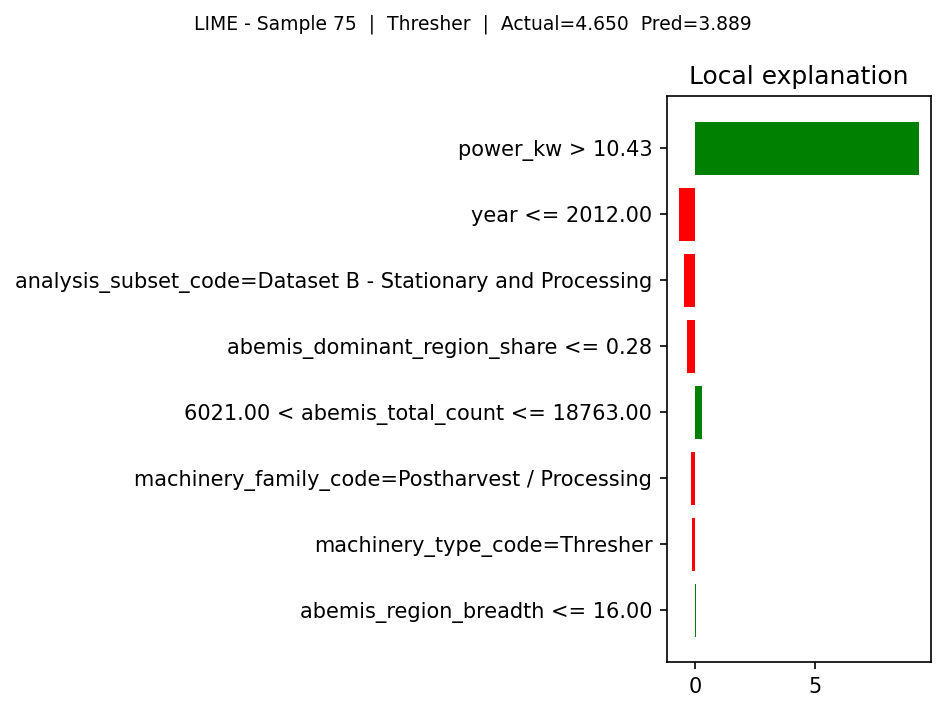
\includegraphics[width=0.85\linewidth]{lime_example_8.png}
  \caption{LIME local explanation --- example record 8.}
\end{figure}

\begin{figure}[H]
  \centering
  
\includegraphics[width=0.85\linewidth]{lime_example_9.png}
  \caption{LIME local explanation --- example record 9.}
\end{figure}

%% ─────────────────────────────────────────────────────────────────────────────
\section*{Appendix D: Descriptive Analytics}

The following figures summarize the AMTEC dataset analytics used during exploratory data analysis and feature engineering. All figures are generated from the 378 cleaned AMTEC records.

\begin{figure}[H]
  \centering
  
\includegraphics[width=0.85\linewidth]{average_fuel_by_machinery_family.png}
  \caption{Average fuel consumption (L/h) by machinery family. Harvest machinery and mobile field machinery show the highest average consumption, consistent with their typically larger engine power ratings.}
\end{figure}

\begin{figure}[H]
  \centering
  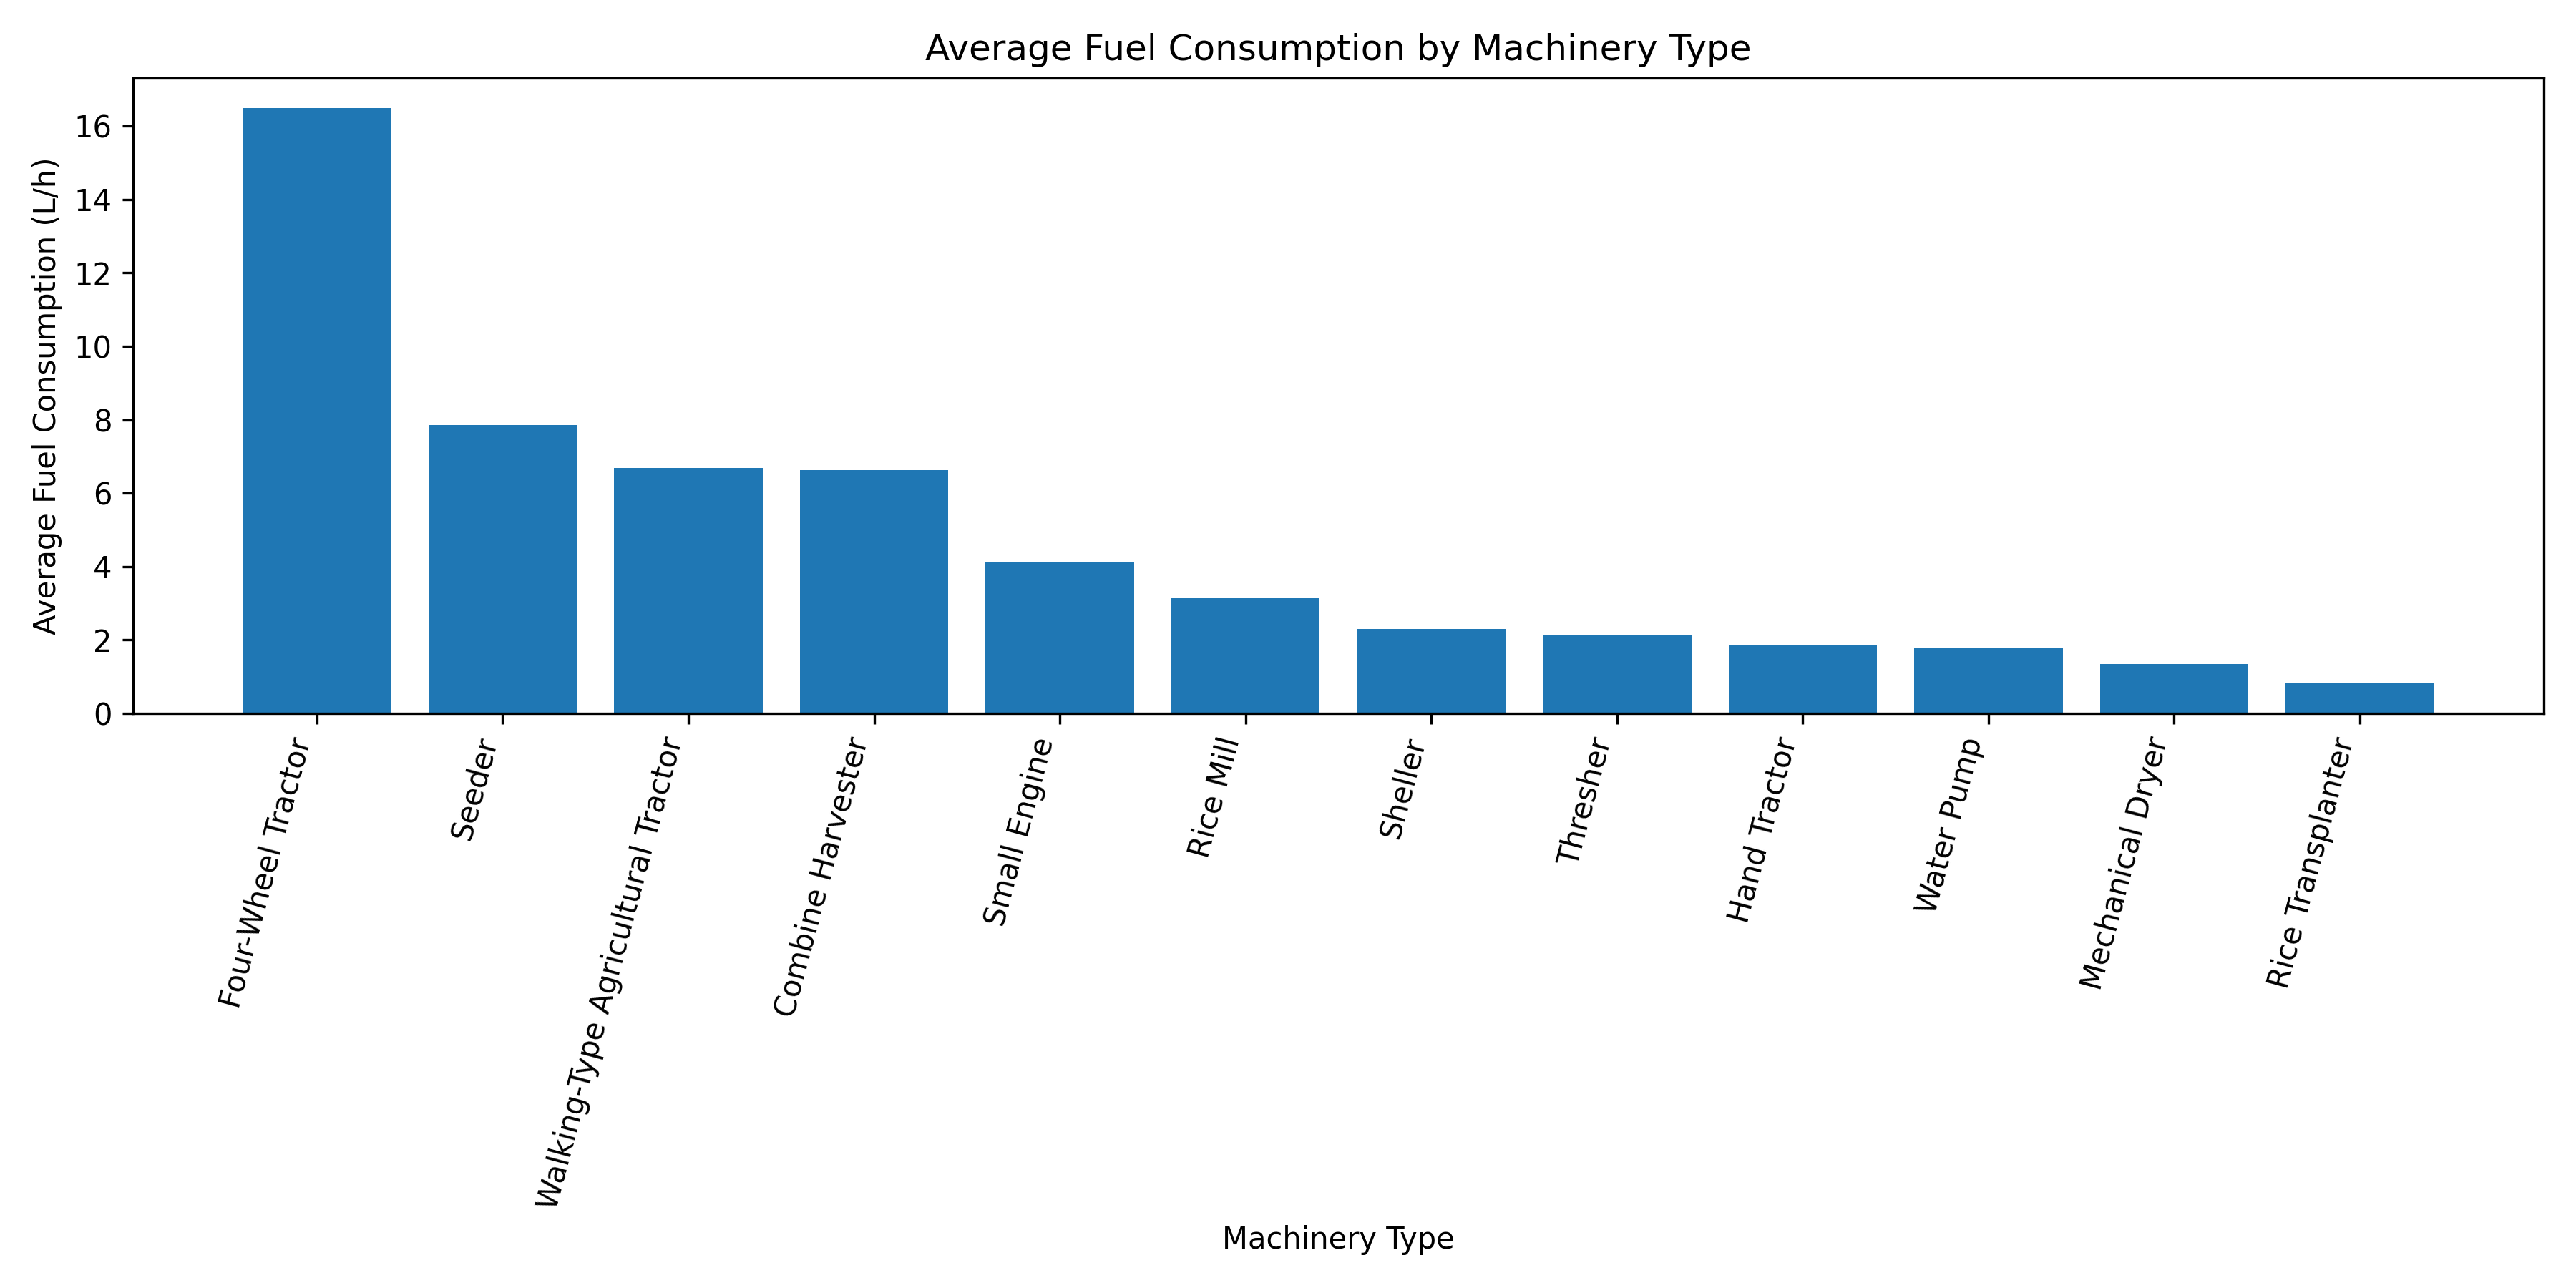
\includegraphics[width=0.85\linewidth]{average_fuel_by_machinery_type.png}
  \caption{Average fuel consumption (L/h) by machinery type. Combine harvesters and four-wheel tractors lead within their respective families.}
\end{figure}

\begin{figure}[H]
  \centering
  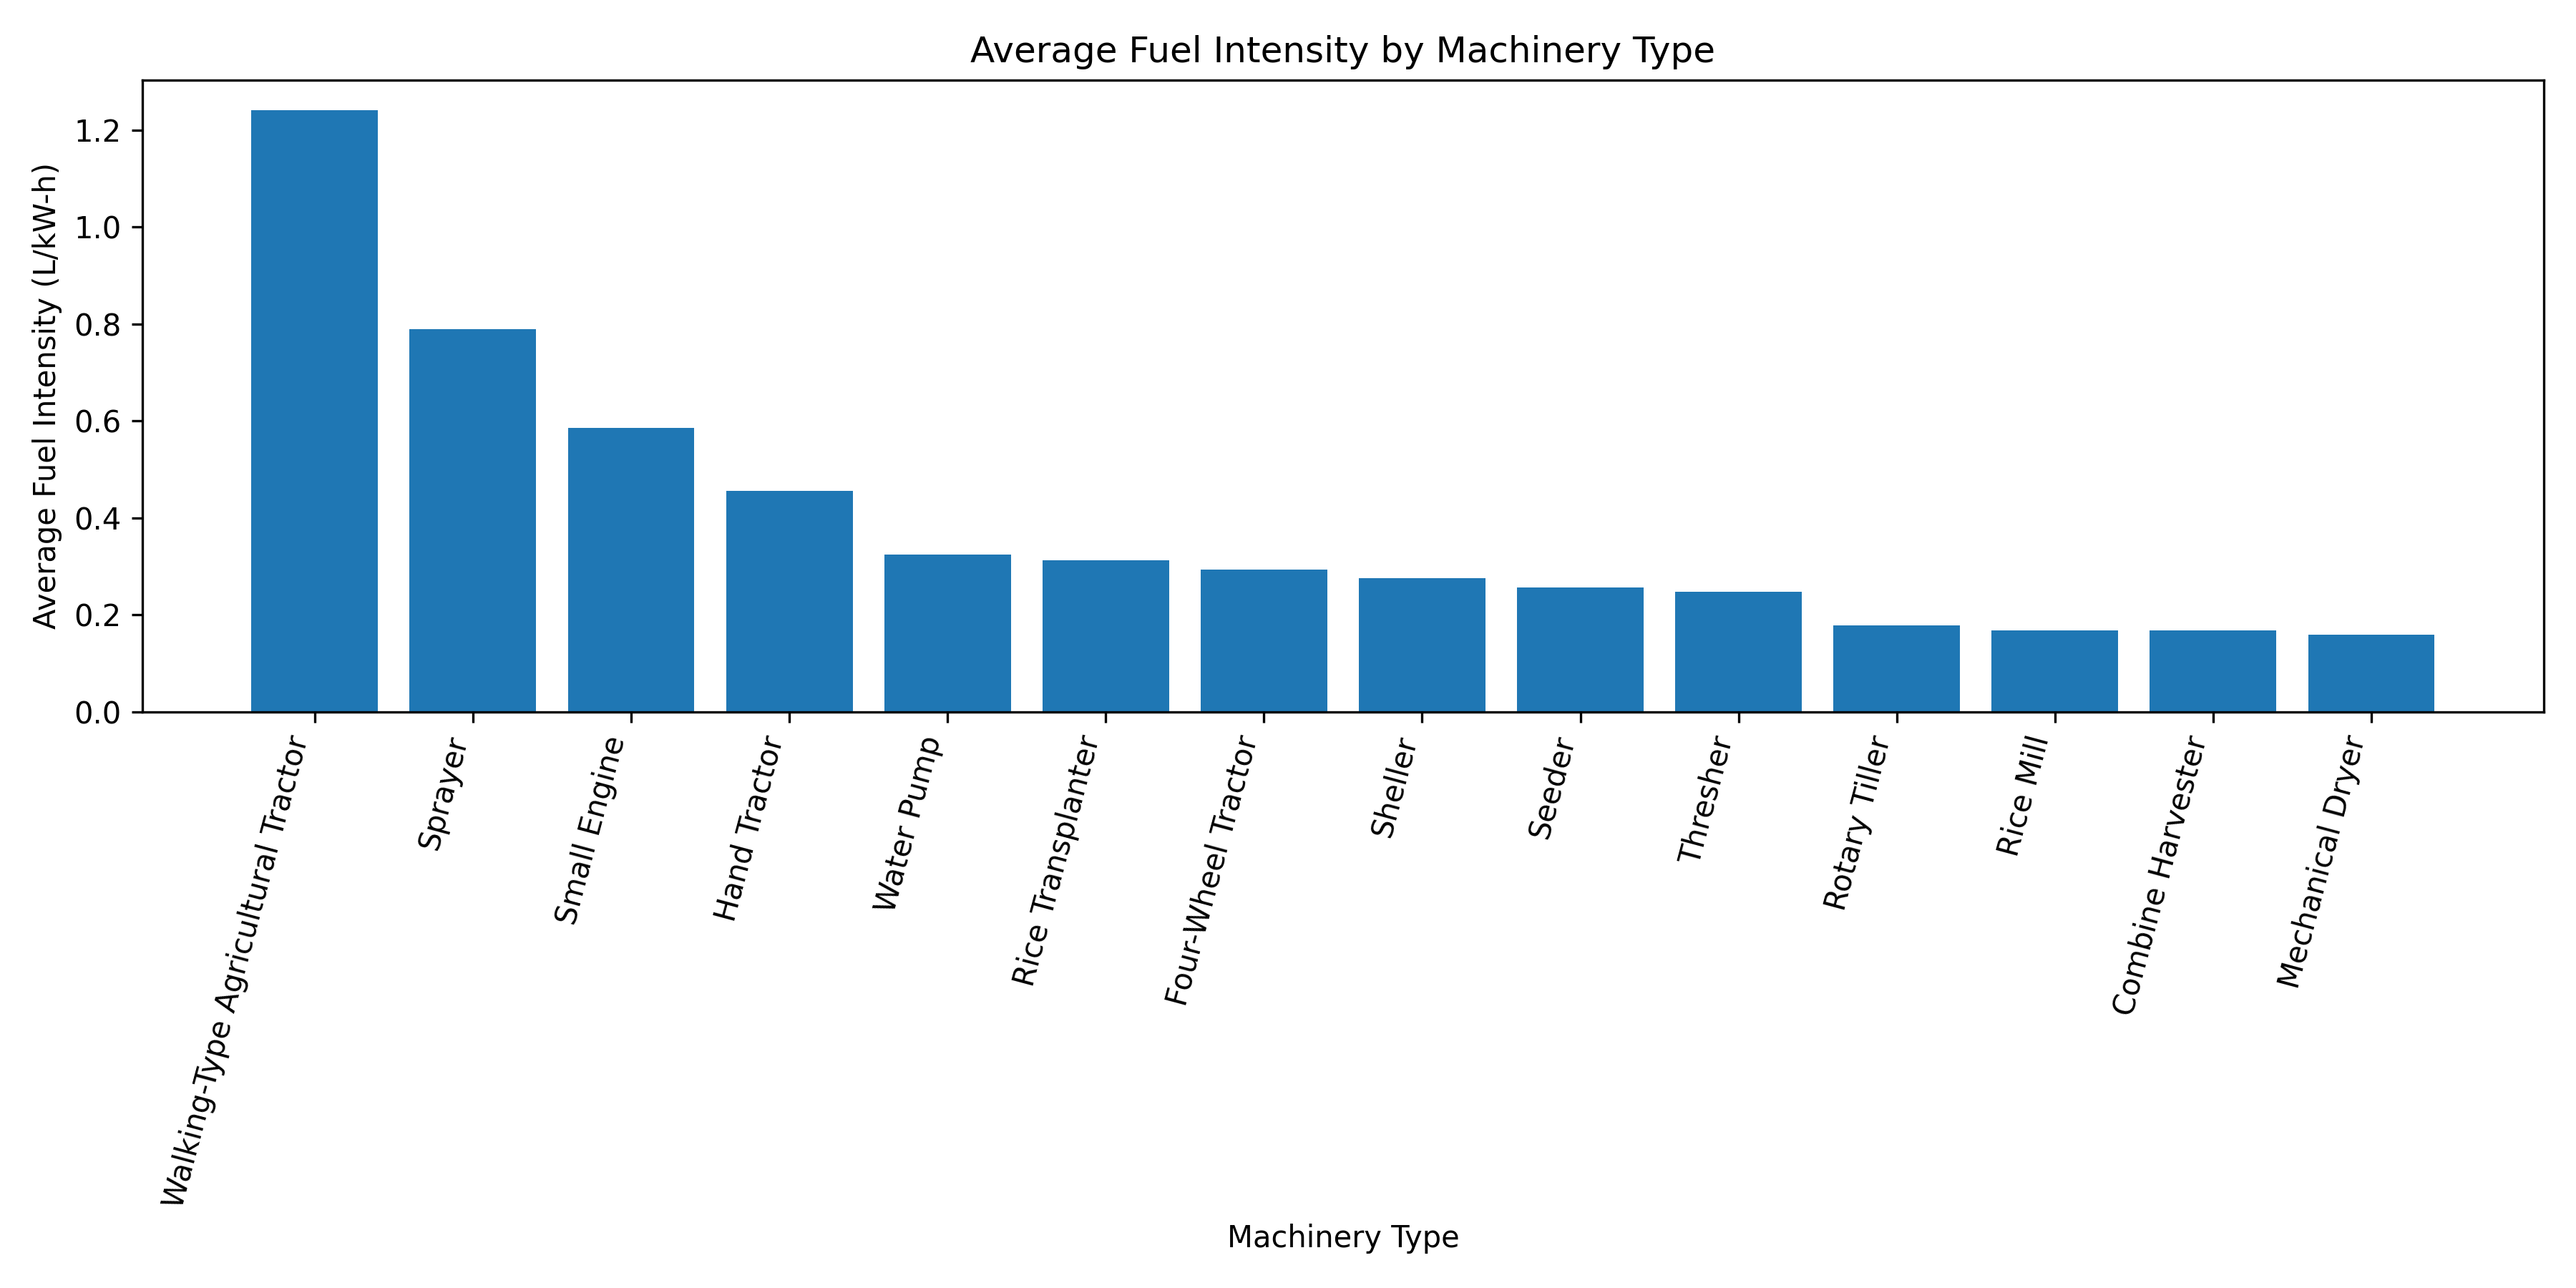
\includegraphics[width=0.85\linewidth]{fuel_intensity_by_machinery_type.png}
  \caption{Fuel intensity (L/h per kW rated power) by machinery type, highlighting operational efficiency differences across machinery categories.}
\end{figure}

\begin{figure}[H]
  \centering
  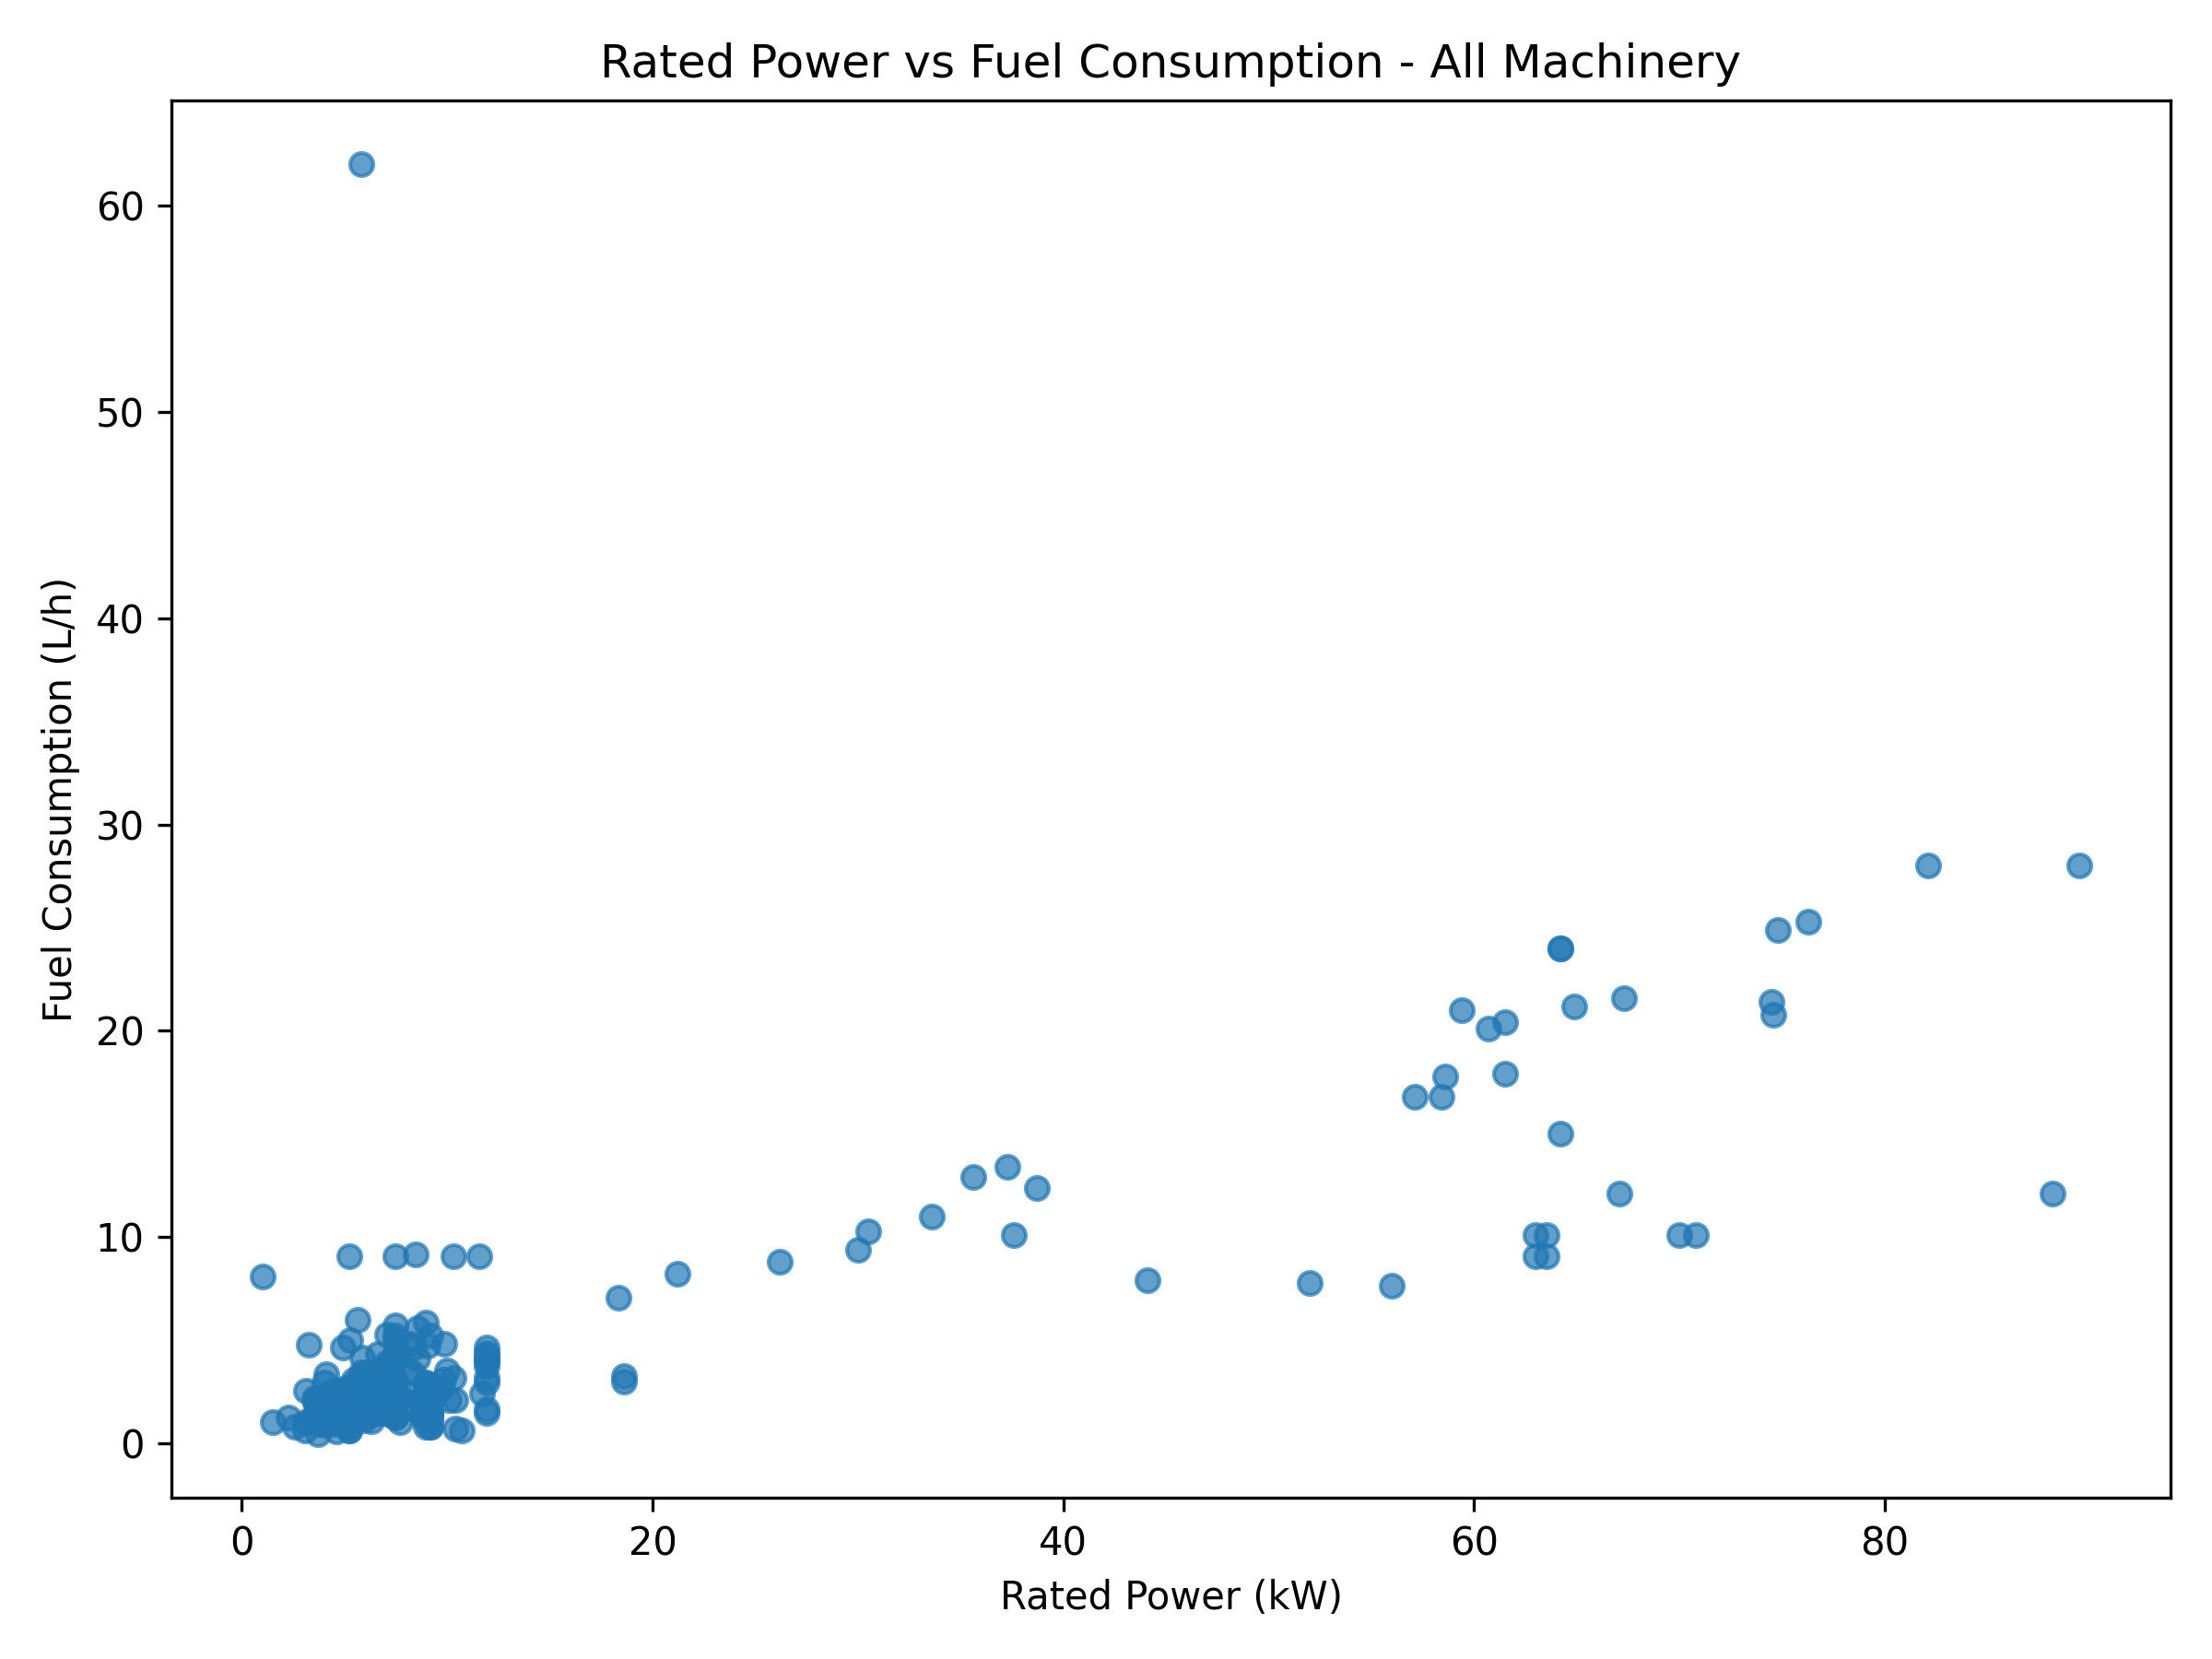
\includegraphics[width=0.85\linewidth]{power_vs_fuel_all.png}
  \caption{Scatter plot of rated power (kW) vs.\ fuel consumption (L/h) for all 378 records. A strong positive relationship is visible, consistent with the SHAP finding that \texttt{power\_kw} is the dominant predictor.}
\end{figure}

\begin{figure}[H]
  \centering
  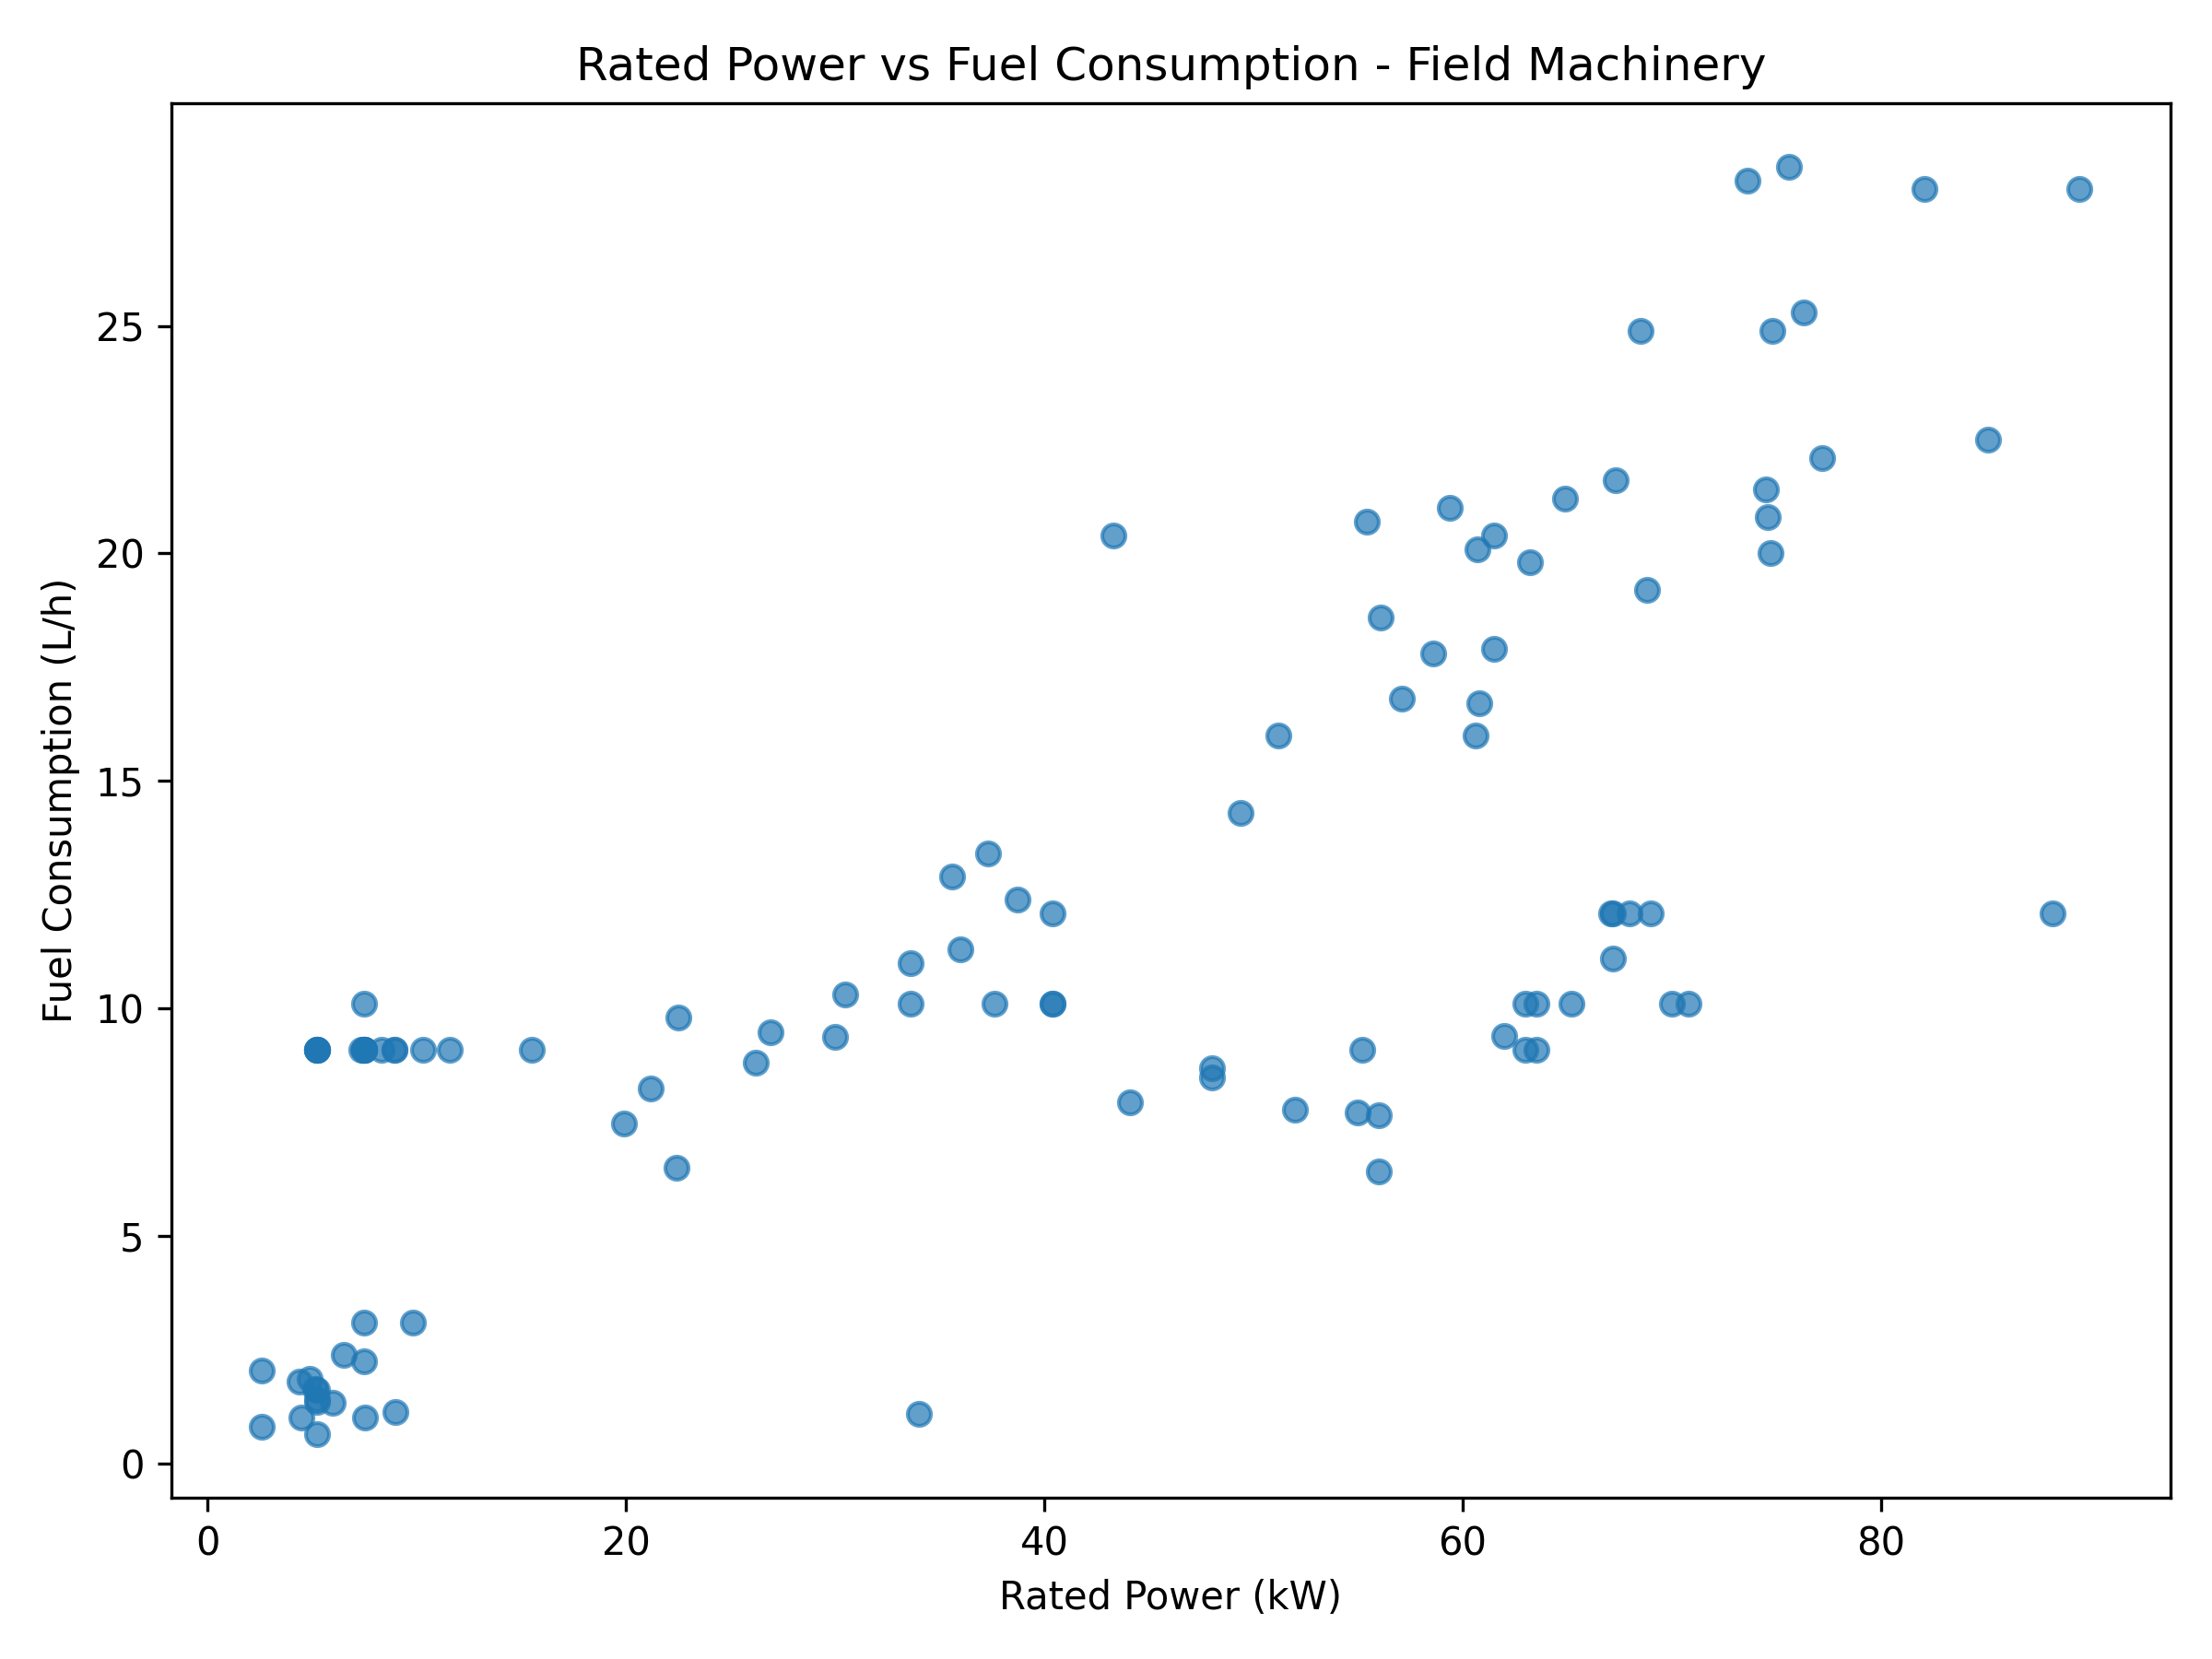
\includegraphics[width=0.85\linewidth]{power_vs_fuel_field_machinery.png}
  \caption{Scatter plot of rated power (kW) vs.\ fuel consumption (L/h) for mobile field machinery only (tractors, tillers). The subset shows a tight linear trend, supporting the quadratic OLS enrichment within this group.}
\end{figure}

\end{document}
